%%%%%
%%
%% Sample document ``thesis.tex''
%%
%% Version: v0.2
%% Authors: Jean Martina, Rok Strnisa, Matej Urbas
%% Date: 30/07/2008
%%
%% Copyright (c) 2008-2011, Rok Strniša, Jean Martina, Matej Urbas
%% License: Simplified BSD License
%% License file: ./License
%% Original License URL: http://www.freebsd.org/copyright/freebsd-license.html
%%%%%

% Available documentclass options:
%
%   <all `report` document class options, e.g.: `a5paper`>
%   withindex   - enables the index. New index entries can be added through `\index{my entry}`
%   glossary    - enables the glossary.
%   techreport  - typesets the thesis in the technical report format. firstyr     - formats the document as a first-year report. times       - uses the `Times` font. backrefs    - add back references in the Bibliography section
% For more info see `README.md`
\documentclass[withindex,glossary,openany]{cam-thesis}

% Citations using numbers
\usepackage[numbers]{natbib}

\usepackage{fancyhdr}

\usepackage{lastpage}       % ``n of m'' page numbering
\usepackage{lscape}         % Makes landscape easier

\usepackage{verbatim}       % Verbatim blocks
\usepackage{listings}       % Source code listings
\usepackage{epsfig}         % Embed encapsulated postscript
\usepackage{array}          % Array environment
\usepackage{array}          % Array environment
\usepackage{enumitem}       % Required by Tom Johnson's exam question header

\usepackage{hhline}         % Horizontal lines in tables
\usepackage{siunitx}        % Correct spacing of units
\usepackage{amsmath}        % American Mathematical Society
\usepackage{amssymb}        % Maths symbols
\usepackage{amsthm}         % Theorems

\usepackage{ifthen}         % Conditional processing in tex
\usepackage{tabularx}
\usepackage{booktabs}

\usepackage[skip=0.5cm]{parskip}

\usepackage[top=3cm,
            bottom=3cm,
            inner=2cm,
            outer=2cm]{geometry}

% If you have any additional \usepackage commands, or other
% macros or directives, put them here.  Remember not to edit
% files in the template directory because any changes will
% be overwritten when template updates are issued.
\usepackage{float,graphicx}
\usepackage{amsmath}
\usepackage{amssymb}
\usepackage{caption}
\usepackage{subcaption}
\usepackage{wrapfig}
\usepackage{listings}

%\usepackage[numbers]{natbib}
\usepackage[nottoc,notlot,notlof]{tocbibind}
\bibliographystyle{unsrtnat}

\lstset{
	basicstyle=\ttfamily,
	literate={~} {$\sim$}{1}
}

\newcommand{\repeatcaption}[2]{%
  \renewcommand{\thefigure}{\ref{#1}}%
  \captionsetup{list=no}%
  \caption{#2 (repeated from page \pageref{#1})}%
  \addtocounter{figure}{-1}% So that next figure after the repeat gets the right number.
}

\usepackage[absolute,overlay]{textpos}

\newcolumntype{C}{>$c<$}
\graphicspath{ {./images/} }

\newcommand{\notimplies}{%
  \mathrel{{\ooalign{\hidewidth$\not\phantom{=}$\hidewidth\cr$\implies$}}}}
\newcommand{\Mod}[1]{\ (\mathrm{mod}\ #1)}
\newcommand{\Z}{\mathbb{Z}}
\newcommand{\R}{\mathbb{R}}
\newcommand{\Q}{\mathbb{Q}}
\newcommand{\N}{\mathbb{N}}


%%%%%%%%%%%%%%%%%%%%%%%%%%%%%%%%%%%%%%%%%%%%%%%%%%%%%%%%%%%%%%%%%%%%%%%%%%%%%%%%
%% Thesis meta-information
%%


\pagenumbering{gobble}
%% The title of the thesis:
\title{Delay-Tolerant Link-State Routing}

%% The full name of the author (e.g.: James Smith):
\author{Ben Andrew}

%% College affiliation:
\college{Magdalene College}

%% College shield [optional]:
\collegeshield{CollegeShields/Magdalene}

%% Submission date [optional]:
% \submissiondate{November, 2042}

%% You can redefine the submission notice [optional]:
\submissionnotice{This dissertation is submitted for Part II of the Computer Science Tripos in 2022}

%% Declaration date:
\date{6th May, 2022}

%% PDF meta-info:
\subjectline{Computer Science}

%%%%%%%%%%%%%%%%%%%%%%%%%%%%%%%%%%%%%%%%%%%%%%%%%%%%%%%%%%%%%%%%%%%%%%%%%%%%%%%%
%% Contents:
%%
\begin{document}

%%%%%%%%%%%%%%%%%%%%%%%%%%%%%%%%%%%%%%%%%%%%%%%%%%%%%%%%%%%%%%%%%%%%%%%%%%%%%%%%
%% Title page, abstract, declaration etc.:
%% -    the title page (is automatically omitted in the technical report mode).
\frontmatter{}

%%%%%%%%%%%%%%%%%%%%%%%%%%%%%%%%%%%%%%%%%%%%%%%%%%%%%%%%%%%%%%%%%%%%%%%%%%%%%%%%
%% Dissertation body:
%%

%%%%%%%%%%%%%%%%%%%%%%%%%%%%%%%%%%%%%%%%%%%%%%%%%%%%%%%%%%%%%%%%%%%%%%%%%%%%%%%%
%% Introduction
%%

\listoffigures

%\lstlistoflistings

\pagebreak

\chapter{Introduction}

\pagenumbering{arabic}

Despite the best efforts of network engineers, achieving reliable communications using traditional routing protocols is inefficient and impractical in many situations. In environments with low network-level reliability, such as remote or developing regions, protocols like OSPF can have large packet drop rates or even provide no end-to-end communication whatsoever. The retransmission costs required to fix this can place strain on already limited resources.

This project aims to evaluate delay-tolerant modifications made to a link-state routing protocol for network environments with low reliability. It is motivated by similar conditions seen in network infrastructure in remote developing regions, where issues such as unreliable power can cause severe and unpredictable drops in packet delivery \cite{DEMMER2007}. I show how modifications made to the routing protocol can reduce this.


\section{Background and Motivation}

A challenging problem in networking is that of routing packets from one side of the network to another on a path hopping from node to node. A routing protocol describes how routers communicate to distribute information about the network's topology in order for each router to choose optimal paths to other nodes, thus making optimal local forwarding decisions for incoming packets. Link-state protocols \cite{LSR_PROTOCOL} are one of the two main classes of routing protocols and aim for every router in the network to have a full view of the network topology. When a change occurs in the network, that information is propagated outwards from router to router and incorporated into each router's internal representation of the network.

Traditional routing protocols such as OSPF treat failures as final, assuming that the failed link will not come back up anytime soon. If alternate routes exist, these protocols route around the failure to maintain connectivity as much as possible. However, if no alternate routes exist (i.e.\ the network has been partitioned), then no data can be sent at all, and all packets sent after the failure will be dropped.

In environments such as developing regions with unreliable network infrastructure, partitions due to temporary link failures are a common occurrence. In this case, the performance of traditional routing protocols drops dramatically, in some cases preventing end-to-end communication entirely. Retransmission-based solutions such as TCP can somewhat help this but make inefficient use of network resources and can cause considerable packet delays. The routing protocols used in these situations must be designed to compensate for these failures to provide good service.

\section{Delay Tolerant Routing}

I explore one approach to make traditional routing more \textit{delay-tolerant}. I do this by allowing routing paths to be advertised through down links, and by using a \textit{store-and-forward} mechanism \cite{SAF} for packet forwarding where if the link on the outgoing interface is down, any packets incoming to the router that would be forwarded out on that interface are buffered in-memory by the router, seen in Figure~\ref{fig:saf_down}. When the link comes back up, all buffered packets are sent out of the desired interface, as seen in Figure~\ref{fig:saf_up}. These techniques maintain end-to-end connectivity as much as possible and decrease the drop rate of packets dramatically.

\begin{figure}[H]
\centering
\begin{subfigure}{1\textwidth}
  \centering
  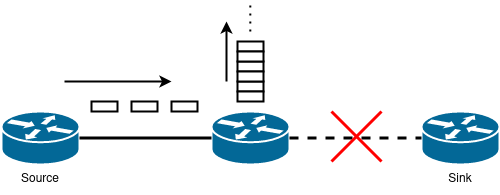
\includegraphics[width=0.57\linewidth]{storeandforward_down}
  \caption{The link is down so the intermediate router buffers packets instead of dropping them.}
  \label{fig:saf_down}
\end{subfigure}
\begin{subfigure}{1\textwidth}
  \centering
  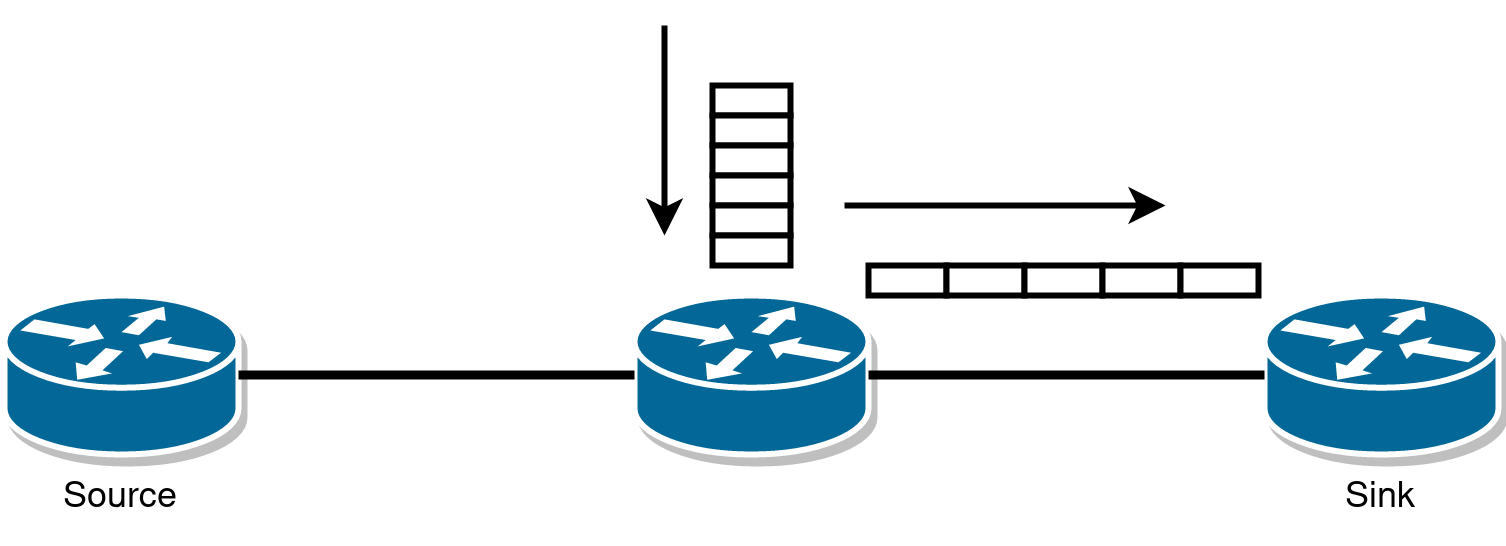
\includegraphics[width=0.57\linewidth]{storeandforward_up}
  \caption{Once the link comes back up the buffered packets are sent by the intermediate router.}
  \label{fig:saf_up}
\end{subfigure}
\caption{Diagram of store-and-forward technique}
\label{fig:saf}
\end{figure}

Figure~\ref{fig:pathalogical} shows a pathological case where anti-correlated link failures mean that there is never an end-to-end connection. Traditional routing techniques will drop all packets, but a store-and-forward technique allows packets to actually be delivered.

\begin{figure}[H]
\centering
\begin{subfigure}{.45\textwidth}
  \centering
  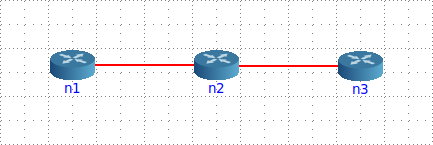
\includegraphics[width=1\linewidth]{pathalogical_topology}
  \label{fig:pathalogical_topology}
\end{subfigure}%
\begin{subfigure}{.55\textwidth}
  \centering
  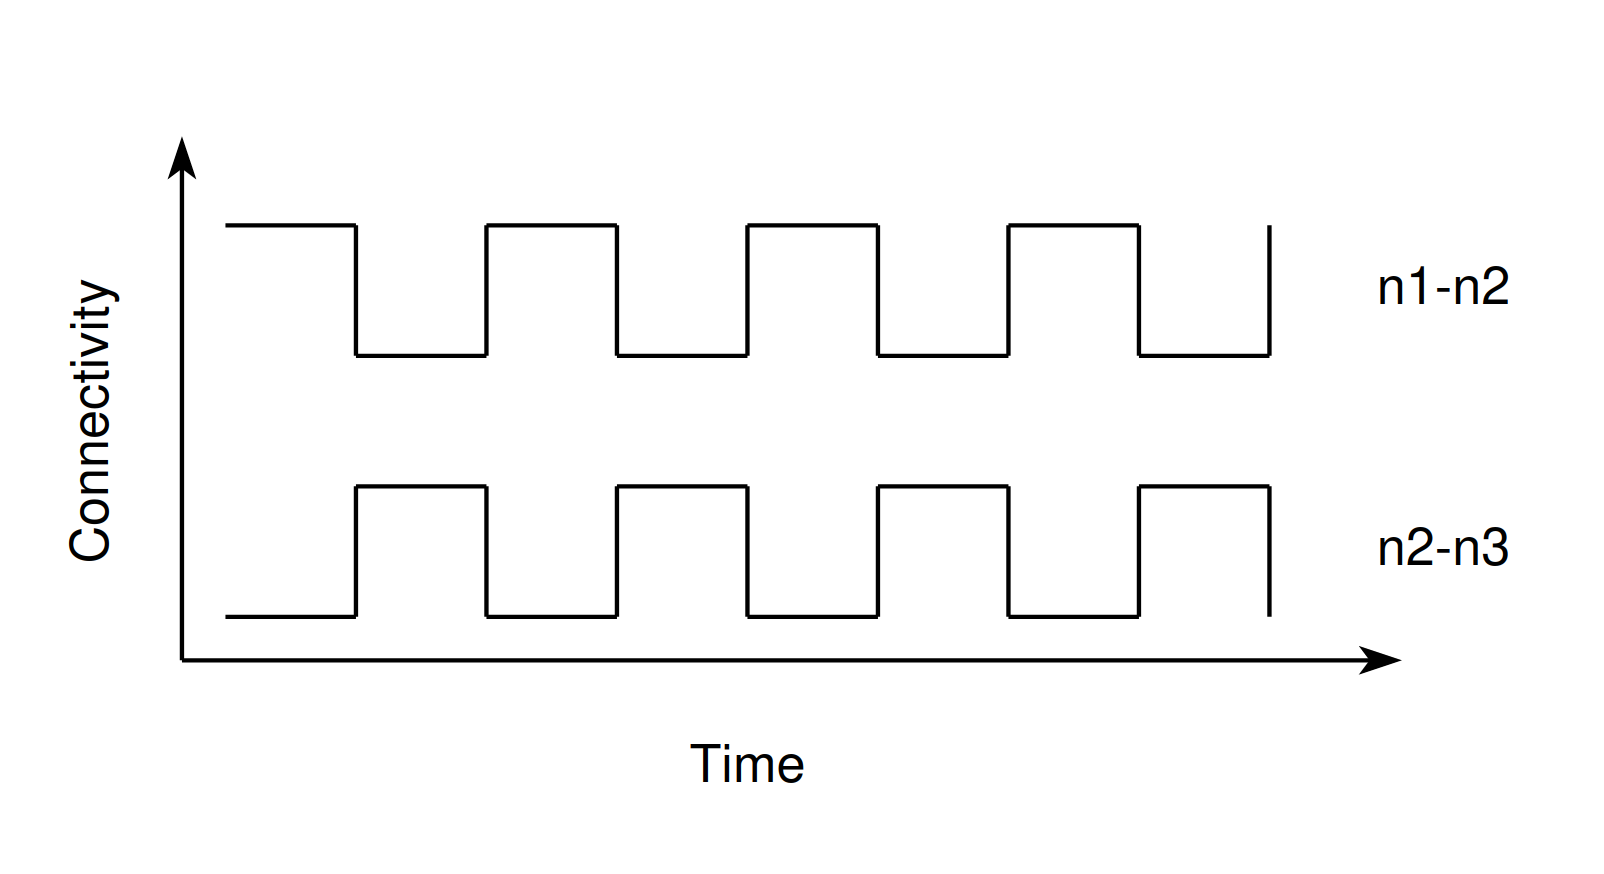
\includegraphics[width=1\linewidth]{pathalogical_graph}
  \label{fig:pathalogical_graph}
\end{subfigure}
\caption{Pathological case with no end-to-end connection}
\label{fig:pathalogical}
\end{figure}

When considering multiple link failures occurring along a path at once, the total time where an end-to-end connection exists can drop greatly. When every router along the path has store-and-forward capabilities, the network becomes far more resistant to failures, giving the best possible service to users given the unreliable environment.

\section{Objectives of the Project}

In this project I produce two routing-layer protocols, \textit{Link-State Routing} (LSR) and \textit{Delay-Tolerant Link-State Routing} (DTLSR); I compare their performance in a number of scenarios that are common in unreliable network environments, focusing on delay and packet delivery rate.

To have control over the behaviour of the protocols both are implemented from scratch in C, with the design based on the OSPF protocol \cite{OSPF}. I perform the evaluation by running the protocols on an industry-grade network emulator \cite{CORE} that provides a realistic testing environment with full control over the network properties; this is detailed in section~\ref{sec:core}.

\subsection{Results}

DTLSR significantly decreases the drop rate of packets over networks with frequent partitions. In cases where the network is partitioned 90\% of the time, I show that DTLSR achieves ten times the packet delivery rate of LSR. Even when a backup link exists, my evaluation shows that DTLSR still reduces the packet drop rate by at least half. I also experimentally show cases with multiple correlated link failures where LSR achieves zero packet delivery, but DTLSR delivers more than 70\% of packets.

\section{Related Work}

There has been much research into \textit{mobile ad-hoc networks} (MANETs) \cite{ABOLHASAN2004}, where mobile nodes physically move around and have intermittent and unpredictable connectivity with other nodes. This mobility requires a dramatic change in network protocol design, and ideas have been explored, such as flooding via relay nodes \cite{CLAUSEN2003}, taking advantage of clustering \cite{ONUR2022}, and even implementing overlay networks to homogenise multiple subnets that use completely heterogeneous network stacks \cite{SCOTT2007}. Of relevance is the \textit{schedule-aware} routing technique, where the contact schedules of pairs of nodes are known and can be exploited \cite{GARETTO2009}. For example, this is used in space networks where one knows the exact time that two satellites will pass by each other in their orbits and send the data on that prediction.

For our situation, this is not necessary as link failures in a mobile network are usually due to topology changes \cite{DIVECHA2007}. Networks in developing regions have largely static topologies with modem or satellite links where link failures, primarily due to congestion or unreliable power, do not imply that the topology has changed \cite{DEMMER2007}. When the failure is resolved, the topology will be the same as before. Thus, one can use a well-understood link-state paradigm with comparatively minor modifications. There is of course a large design space to explore \cite{FARRELL2006}, but I choose to make smaller modifications which makes deployment far easier and minimises wasted resources from unnecessary features. It's desirable to use as many off-the-shelf components as possible to reduce cost, a critical requirement of infrastructure in environments like these.

\chapter{Preparation}

\section{Link vs Node Failures}
\label{sec:link_vs_node_failures}

As DTLSR is designed to respond well to network failures, choosing the types of failures for the evaluation is critical to provide an accurate comparison to LSR. I consider two types of failures, \textit{link} and \textit{node}. Link failures prevent two functioning nodes from communicating with each other at the link-level, shown in Figure~\ref{fig:link_failure}. When no alternate route exists, recovery requires the link to be restored, at which point communication continues as normal.

Node failures are more serious, with nodes often having multiple connections; failure of a central router may disrupt communication between many nodes, as seen in Figure~\ref{fig:node_failure}. Also consider that the link-state representation of the network is stored in memory: link-state information that has been propagated across the entire network will be lost. Thus, recovery involves not just the node restarting but also reaquiring the link-state from neighbours, increasing recovery time and complexity.

\begin{figure}[H]
\centering
\begin{subfigure}{0.5\textwidth}
	\centering
	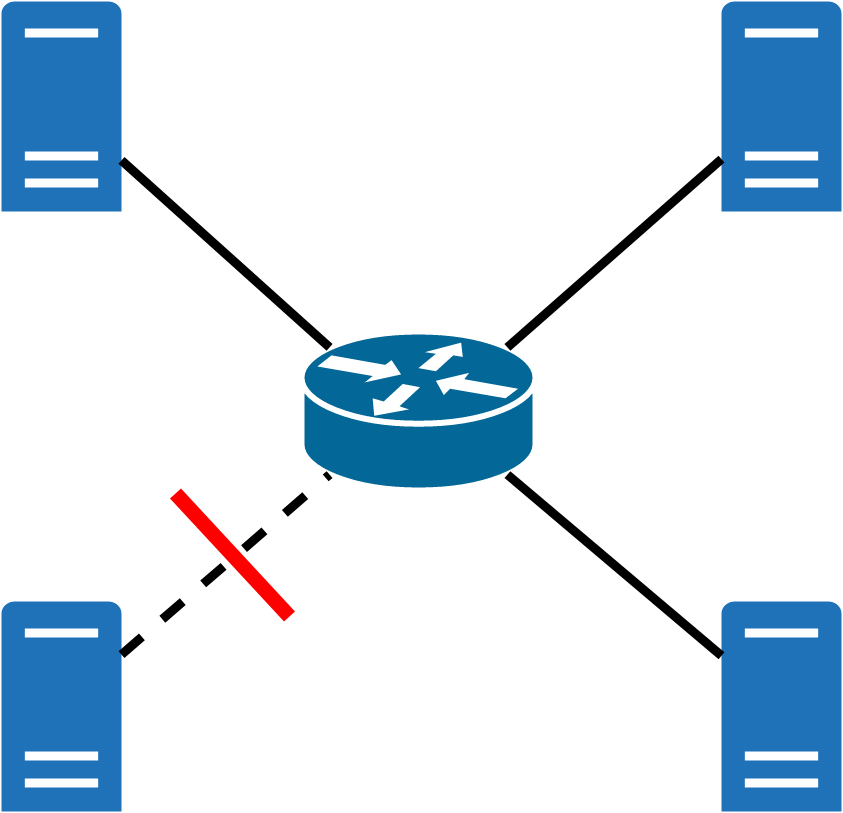
\includegraphics[width=0.5\textwidth]{link_failure}
	\captionof{figure}{Link failure}
	\label{fig:link_failure}
\end{subfigure}%
\begin{subfigure}{0.5\textwidth}
	\centering
	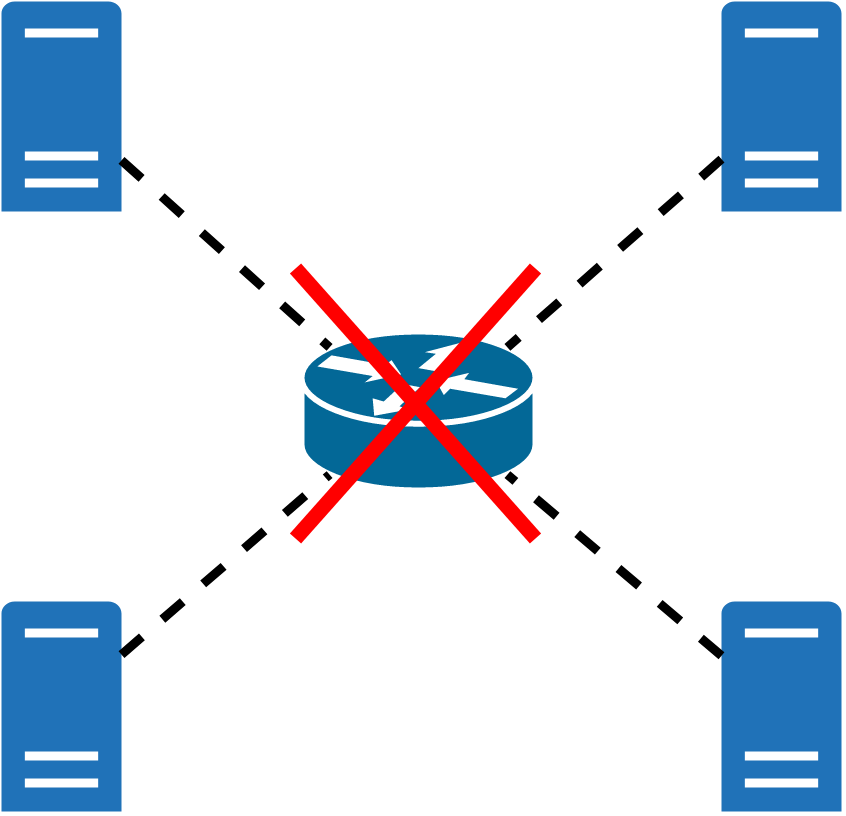
\includegraphics[width=0.5\textwidth]{node_failure}
	\captionof{figure}{Node failure}
	\label{fig:node_failure}
\end{subfigure}
\captionof{figure}{Types of network failures}
\end{figure}

To a neighbour, the symptoms of a failed node are identical to a link failure due to the heartbeat system that I use being disrupted in both cases. Link failures may occur due to wireless interference or faulty cables, and node failures can occur due to intermittent power.

\section{Common Open Research Emulator (CORE)}
\label{sec:core}

CORE \cite{CORE} is a network emulator that models nodes as lightweight Unix virtual machines, complete with filesystems and network interfaces. It comes out of the U.S.\ Naval Research Laboratory and was developed by Boeing Research and Technology. In Figure~\ref{fig:core_topology} we see an example topology in the CORE GUI, showing virtual routers and hosts along with their IP addresses. Listing~\ref{core_filesystem} shows an example of a virtualised file-system of node \texttt{n1}; boot scripts and log files of the DTLSR (\texttt{dtlsr}) and Heartbeat (\texttt{hbt}) protocols are visible. Nodes communicate via virtualised interfaces, connected by bridges emulating physical links; Listing~\ref{core_interfaces} shows an example of this.

\begin{center}
\begin{minipage}{0.9\textwidth} \centering
	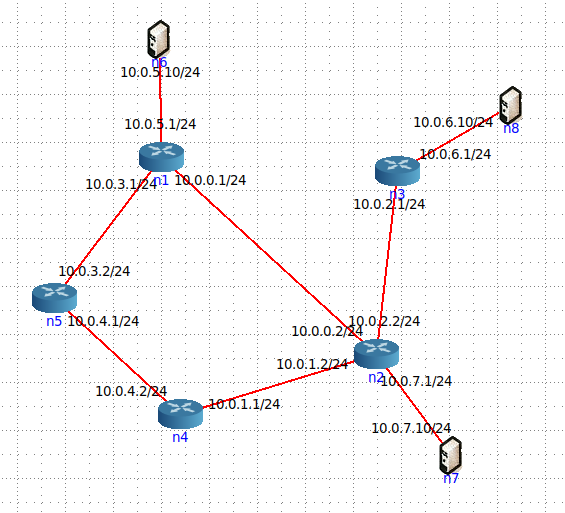
\includegraphics[width=0.65\textwidth]{core_topology}
	\captionof{figure}{Example emulated network in the CORE GUI}
	\label{fig:core_topology}
\end{minipage}
\end{center}

Programs can be written for these nodes and run as Unix processes via a Python API. These processes are able to send and receive data through the emulated network via standard Unix socket programming. The emulated routers contain default routing protocol implementations, such as OSPFv2 and -v3 from the Quagga protocol suite \cite{QUAGGA}, which can be disabled and replaced by custom implementations. As well as this, standard network testing tools like \texttt{ping} can be run on emulated endpoint hosts, making testing and evaluation of the network simple: in the topology in Figure~\ref{fig:core_topology} I could run \texttt{ping 10.0.5.10} from the node \texttt{n7}, sending pings between \texttt{n7} and \texttt{n6}.

Link properties such as delay and loss can be programmatically customised through the Python API. This aids greatly in evaluation, allowing me to simulate network partitions and other network events. In Figure~\ref{fig:core_topology} if I disabled link \texttt{n1-n2} the pings going between \texttt{n7} and \texttt{n6} would have to be rerouted through \texttt{n5} and \texttt{n4}.

An interesting point is that all of the VMs are run in real-time on a single host, sharing the host operating system's clock; the performance of the simulated network is thus dependent on the performance of the machine it is running on. I therefore take great care to create a reliable and statistically sound testing environment, for example setting processor priority, not running other programs, and taking baseline measurements to compare against. However the clock sharing is also an advantage for evaluation, as when deriving the time between events on different virtual machines I don't need to account for any clock drift; the time difference will be as exact as if they were the same machine. This will make evaluation easier and more accurate, reducing the error.

\begin{minipage}{1\textwidth} \centering
\begin{lstlisting}[label=core_filesystem, frame=tb, caption=Example of a virtualised file-system]
ben@ben-laptop:/tmp/pycore.1/n1.conf$ ls -lh
total 40K
-rw-r--r-- 1 root root   98 Apr 16 14:43 defaultroute.sh
-rw-r--r-- 1 root root  103 Apr 16 14:43 hbtboot.sh
-rw-rw-rw- 1 root root 2.1K Apr 16 14:44 hbt.log
-rw-r--r-- 1 root root  798 Apr 16 14:43 ipforward.sh
-rw-r--r-- 1 root root   91 Apr 16 14:43 dtlsrboot.sh
-rw-rw-rw- 1 root root   61 Apr 16 14:43 dtlsr.log
\end{lstlisting}
\end{minipage}

\begin{minipage}{1\textwidth} \centering
\begin{lstlisting}[label=core_interfaces, frame=tb, caption=Virtualised network interfaces and bridges]
ben@ben-laptop:~$ nmcli device status
DEVICE          TYPE      STATE         CONNECTION
b.10.1          bridge    connected     b.10.1
b.11.1          bridge    connected     b.11.1
b.7.1           bridge    connected     b.7.1
b.8.1           bridge    connected     b.8.1
b.9.1           bridge    connected     b.9.1
veth1.0.1       ethernet  unmanaged     --
veth1.1.1       ethernet  unmanaged     --
veth1.2.1       ethernet  unmanaged     --
veth2.0.1       ethernet  unmanaged     --
veth2.1.1       ethernet  unmanaged     --
veth2.2.1       ethernet  unmanaged     --
veth3.0.1       ethernet  unmanaged     --
veth4.0.1       ethernet  unmanaged     --
veth5.0.1       ethernet  unmanaged     --
veth6.0.1       ethernet  unmanaged     --
\end{lstlisting}
\end{minipage}

\pagebreak

\section{Software Engineering Tools and Techniques}

\subsection{Requirements Analysis}

The success criteria revolve around creating two routing protocols, and comparing their performance in a number of metrics. In order to meet these criteria, the implementation must include both the tools to run the protocols as well as tools to evaluate it. These can be further split into more specific deliverables,
specified in Table~\ref{table:requirements}.

\begin{table}[H]
\centering
\begin{tabular}{@{}p{0.75\textwidth}l@{}}\toprule
\Large\textbf{Requirement} & \Large\textbf{Priority} \\
\midrule
\midrule
\textbf{Implementation} & \\
\midrule
Appropriate link-state representation of the network & Fundamental \\\addlinespace[0.2em]
Implementation of LSR protocol & Fundamental \\\addlinespace[0.2em]
Making delay-tolerant modifications to LSR to produce DTLSR & Fundamental \\\addlinespace[0.2em]
Implement DTLSR link metric for comparison with alternate routes & Preferable \\\addlinespace[0.2em]
\midrule
\midrule
\textbf{Evaluation} & \\
\midrule
Analysis and comparison of LSR and DTLSR & Fundamental \\\addlinespace[0.2em]
CORE testing infrastructure: data logging, virtual commands, etc. & Preferable \\\addlinespace[0.2em]
CORE automatic network generation from config file & Preferable \\\addlinespace[0.2em]
\bottomrule
\end{tabular}
\caption{Requirements specification.}
\label{table:requirements}
\end{table}

\subsection{Tools}

\paragraph{Programming Languages:}

I used \textbf{C} because of extensive previous experience in internships and the Part 1B course, and in order to have low-level access to Unix system calls. As well as this industry-grade routing protocols are generally written in C or assembly, and I wanted to emulate this as much as possible. I used \textbf{Python} to interact with the CORE API, for scripting the testing environment used to evaluate and develop the routing protocols. The Python API is the only one provided, so it was a natural choice. I also used Python extensively to analyse and plot the collected data.

\paragraph{Libraries:}

I used \textbf{libpcap} and its command-line equivalent \textbf{tcpdump} \cite{TCPDUMP} for buffering received packets and storing them on the router when the outgoing link was down. I used \textbf{tcpreplay} \cite{TCPREPLAY} to send the packets buffered by the tools above out onto the outgoing link when it came back up.

\paragraph{Version Control and Backup:}

I used the \textbf{Git} version control tool, with the repository backed up on the \textbf{GitHub} platform. The repository was also backed up on an external hard drive.

\paragraph{Building and Testing:}

I used the \textbf{CMake} build system for C, which allows easy inclusion of dependencies such as libpcap and check, and the generation of multiple executables in the same project, even from the same source files. It also provides platform independence. I used the \textbf{Check} unit-testing framework for C.

\paragraph{Integrated Development Environment:}

I used \textbf{Visual Studio Code} as the main development environment, programming in both C and Python. It provides a syntax highlighted text editor along with functionality to easily build and run programs.

\paragraph{Other Tools:}

I used \textbf{CORE version 7.5.2} as it provides a reliable network emulation platform for development and evaluation of network protocols. In particular, it allowed me to disable the existing routing protocols and replace them with my own. I used the \textbf{Packet CAPture (.PCAP)} format, a standard file format for packet data, to store the buffered packets on the router until they could be replayed. It was chosen as tcpdump and tcpreplay understand this format natively.


\section{Starting Point}

This project does not build on any other code/project, but only makes use of common tools and libraries such as libpcap, CORE, and matplotlib (for plotting graphs in the dissertation). CORE comes packaged with standard routing protocol implementations of OSPFv2 and v3, however I disable these completely and do not use them as a starting point for my code, neither for inspiration nor code snippets.

\section{Summary}

The concepts and algorithms required for the dissertation were mostly covered in Part IB Computer Networking, but the delay-tolerant protocol modifications were not included in the course and I had no prior experience with them. Previous experience with C came from the Part IB course as well as a summer internship doing embedded development.

\chapter{Implementation}

This chapter discusses the implementation of two routing protocols, LSR and DTLSR. The initial design of LSR is described in section~\ref{sec:lsr_design}, and the modifications made to produce DTLSR are described in section~\ref{sec:dtlsr_design}. Each protocol is composed of link-layer systems for detecting link failure and links coming back up, integration of this information into an internal graph representation of the network, and a network-layer mechanism for propagating this information over the entire network.

Also implemented is a way for each router to use this information to generate shortest paths to every other node, aggregating this information to modify the routing table accordingly. Significant effort was put into the delay-tolerant modifications in DTLSR, with a local packet buffering system for link-failure tolerance, and a sophisticated metric for comparing the reliability of links when alternate routes exist.

\section{Link-State Routing Design}
\label{sec:lsr_design}

In this section I first show an overview of the traditional link-state protocol, detailing how it recovers from failed nodes (section~\ref{subsec:node_failure}), how link-state is shared between routers (sections~\ref{subsec:merge_rlsa} \& \ref{subsec:merge_nlsa}), how local and global state is distinguished (section~\ref{subsec:landg_state}), and finally how routes are generated (section~\ref{subsec:route_generation}).

The link-state routing protocol that I implemented is split into two programs, Heartbeat and LSR.  Routers run both programs, and hosts run only Heartbeat.

Heartbeat sends periodic heartbeat messages to all neighbouring nodes, notifying them that the connecting link is still up. The message is received by LSR. Hosts run Heartbeat to notify their gateway router of their existence, so that the router can advertise the corresponding gateway route.

LSR implements the bulk of the protocol. It maintains the link-state graph representation of the network, manipulates the node's routing table, and sends router link-state announcements (rLSAs)\footnote{Router LSAs contain only the local vicinity of the router in question, network LSAs (detailed in section~\ref{subsec:node_failure}) contain the entire network and are used for node recovery.} to neighbours in response to detected changes in the network (detailed in section~\ref{subsec:merge_rlsa}). When I say a link is UP or DOWN I mean the router's logical link-state representation of the network, which is a `lagged' view of its real state. The event loop of LSR is shown in Figure~\ref{fig:flowchart_lsr}, showing responses to different events.

Network changes are detected in one of three ways:
\begin{enumerate}
	\item
	A heartbeat message is received from a neighbour with a DOWN link. I set the link to be UP.
	
	\item
	A heartbeat is not received in time from a neighbour with an UP link. I set the link to be DOWN.
	
	\item
	An rLSA is received from a neighbour. If it contains any information more recent than the router's that causes a change to its network representation when merged in, a change is detected. In this case the router floods this rLSA to its other neighbours, propagating the update across the network.
\end{enumerate}

\begin{figure} \centering
	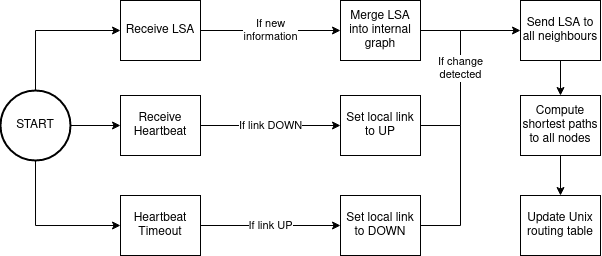
\includegraphics[width=0.9\textwidth]{flowchart_lsr}
	\captionof{figure}{Event loop of LSR}
	\label{fig:flowchart_lsr}
\end{figure}

Both programs lend themselves to an event-driven design, and so I used file descriptors multiplexed with the \texttt{select} Unix system call to detect and respond to events. The \texttt{select} call blocks the process from running until one of the specified file descriptors is ready to be used, at which point the OS gives the process back control along with information about which file descriptor is ready. Using this I can implement a coarse event system. As examples, receiving socket file descriptors trigger as \textit{ready} when data has arrived and is ready to be read, and timer file descriptors trigger as \textit{ready} when the timer has expired. One can see how these can be composed to create a responsive distributed protocol that uses system resources efficiently, rather than just spinning waiting for something to happen.

Heartbeats and rLSAs are received on sockets with distinct ports, allowing them to be differentiated easily by the Unix socket API at the UDP layer. While these are purely link-level communications and as such do not require UDP or even IP information, the socket API is an easy abstraction to use and allows me to reuse code from other parts of the codebase, minimising the possibility of introducing bugs.

A heartbeat message is a UDP packet with only a header and no payload. An rLSA is a UDP packet whose payload is the sending node's graph representation of its immediate network vicinity (it and its neighbours), simply copied into the payload using the \texttt{memcpy} C function.

I use a triggered update system, sending rLSAs to the router's neighbours whenever we detect a change in the network;  this propagates link-state information as quickly as possible to minimise convergence time. I also send only when the router detects changes with respect to its knowledge of the network so that we don't cause infinite looping of updates.

\subsection{Recovery from Node Failure}
\label{subsec:node_failure}

When a node crashes, it loses all of its knowledge about the graph. On rebooting it is desirable to reaquire that knowledge as quickly as possible, so I implement functionality for a node to request from its neighbours not just their localised rLSAs, but their entire network graph all at once, termed a \textit{network link-state announcement} (nLSA). This speeds up the recovery of the node's routing capability significantly, as it doesn't have to wait for triggered rLSAs to be sent from all edges of the network.

On rebooting, a router sends to all of its neighbours an nLSA request, and each neighbour responds by sending back its own nLSA. The router merges these nLSAs together to get the most up-to-date view of the network, generates the correct routes, and then updates the forwarding table.

\subsection{Graph Merging: Router LSAs}
\label{subsec:merge_rlsa}

An rLSA contains information only about the immediate vicinity of the router, represented by a single \texttt{Node} in the representation; merging this information into the graph is thus very simple. I first compare the timestamps of the stored node and rLSA node: if the node's is more recent we do nothing as we have received stale information. If the rLSA node is more recent then I first relay the rLSA to all of the node's other neighbours to propagate the change through the network, and then copy the data in the node into its own graph, incorporating the new information.

\subsection{Graph Merging: Network LSAs}
\label{subsec:merge_nlsa}

A network LSA (nLSA) contains a router's full view of the network, and so merging becomes more involved to make sure it only takes the most recent information. Figure~\ref{fig:lsa} shows an example of a merge, where node A receives an nLSA from node B, and merges it in to get the most up-to-date view of the network. Blue nodes and links are from A, and yellow ones are from B, showing in the output graph which nodes and links were taken from whose graph.

\begin{center}
\begin{minipage}{0.9\textwidth} \centering
	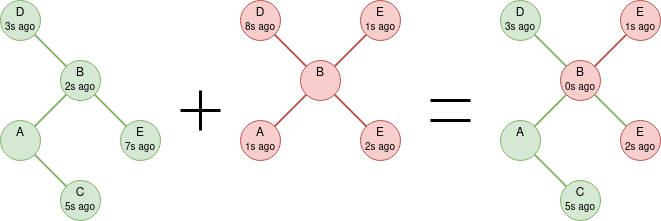
\includegraphics[width=1\textwidth]{lsa}
	\captionof{figure}{Example of link-state graph merging}
	\label{fig:lsa}
\end{minipage}
\end{center}

To allow merging to be simple I treat every node as independent, in particular having the node's list of neighbours included in the node's data structure rather than having a separate list of links indexed by 2-tuples of node IDs. While this doubles the memory cost of a link as I represent it with two directed edges rather than a single undirected one, it means that merging becomes a simple independent pairwise comparison between nodes of the same ID to pick the one with the most recent timestamp, which has an $O(n)$ time complexity in the number of nodes in the graph.

Merging nLSAs is important as after rebooting and sending nLSA requests to all of its neighbours, the node may receive many nLSAs back that must be merged together.

\subsection{Local and Global Link-State}
\label{subsec:landg_state}

I have two levels of representation for my network graph: a minimal global representation of the entire network and a detailed representation of the immediate neighbourhood of the local node. I use the detailed local state to derive metrics for the global state graph that can be efficiently shared with other routers.

For each node in the global graph, I store for each link information like the source IP, neighbour destination IP, the status of the link, the derived metric associated with the link, and a timestamp specifying how old the knowledge of that link is, for merging purposes.

The local graph consists solely of the node along with more in-depth information about links connecting it to its immediate neighbours. Along with all of the information contained in a global node, I also have for each link a timer for timing out heartbeats and the interface which that link goes out on. I take the locally-derived information, disseminate it to the rest of the network via rLSAs, and then feed it into the global graph for making local forwarding decisions.

To help explain the data structures used, an example is shown in Figure~\ref{fig:node_ex}, with the fields of node \texttt{n1} described in detail in Listing~\ref{node_ex_listing}. The global graph is an array of \texttt{Node} structs, and the local graph is a single instance of a \texttt{LocalNode} struct, representing the router itself.

\begin{center}
\begin{minipage}{0.9\textwidth} \centering
	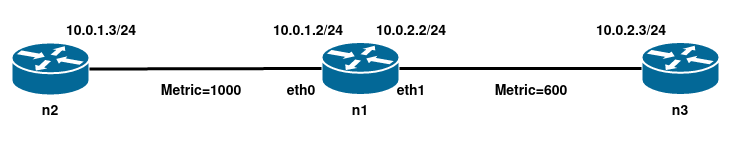
\includegraphics[width=1\textwidth]{node}
	\captionof{figure}{Diagram of stored node and link information}
	\label{fig:node_ex}
\end{minipage}
\end{center}

\begin{minipage}{1\textwidth} \centering
\begin{lstlisting}[language=C, label=node_ex_listing, frame=tb, columns=fullflexible, caption=Partial example of fields of \texttt{Node} and \texttt{LocalNode}]
Node fields:
 neighbour_ids = [2, 3]
 neighbour_ips = [10.0.1.3/24, 10.0.2.3/24]
 source_ips = [10.0.1.2/24, 10.0.2.2/24]
 link_statuses = [UP, UP]
 link_metrics = [1000, 600]

LocalNode fields:
 interfaces = [eth0, eth1]
\end{lstlisting}
\end{minipage}

\subsection{Route Generation}
\label{subsec:route_generation}

I generate routes from the link-state graph, computing shortest paths from the router in question to every other node using Dijkstra's algorithm. From each shortest path I get the next-hop node, which I add to the forwarding table along with the destination IP subnet so that the router knows where to forward incoming packets. Along with adding new routes I also delete old stale routes, which have either been made obsolete by a new, better route, or do not exist anymore due to failure.

Dijkstra's algorithm solves the single-source all-destinations shortest path problem for graphs with non-negative weights, allowing me to choose a metric to judge links against each other. The metric must be additive for \textit{shortest} to be meaningful. Traditional OSPF uses a bandwidth-based metric, but I chose to use the number of hops in the path instead, as delay is more important than throughput in delay-tolerant networks.

With many destinations there exist a large number of forwarding table entries, but this can be reduced by aggregating routes together that share an outgoing interface and IP prefix. As the forwarding table operates by prefix matching, I only need to insert the shared prefix into the table, reducing the number of entries required greatly.

Manipulation of the Unix routing table is done through \texttt{ioctl}, a system call for interacting with OS devices through a file descriptor interface. I pass a flag corresponding to route addition or deletion, along with a \texttt{route} struct containing the route details.

\section{Delay-Tolerant Modifications}
\label{sec:dtlsr_design}

In this section I first show how routers buffer packets in the event of failures (section~\ref{subsec:packet_buffering}), then how the pathfinding algorithm and forwarding table must be modified to support routing through down links (section~\ref{subsec:routing_down_links}), and finally detailing the link metric used to compare down links (section~\ref{subsec:link_metric}).

For the delay-tolerant version of the protocol suite, I replace the LSR executable with DTLSR, keeping Heartbeat the same. DTLSR uses mostly the same source files as LSR, with the delay-tolerant modifications enabled by \texttt{\#ifdef DTLSR} preprocessor switches, as shown in Listing~\ref{preprocessor_switch} where the choice of link metric differs in LSR and DTLSR. DTLSR maintains many of the same implementation design decisions as above with a few additions. Figure~\ref{fig:flowchart_dtlsr} shows the modified event loop of DTLSR, with new stages shown in blue, and existing stages that have been modified shown in yellow.

\begin{center}
\begin{minipage}{0.9\textwidth} \centering
	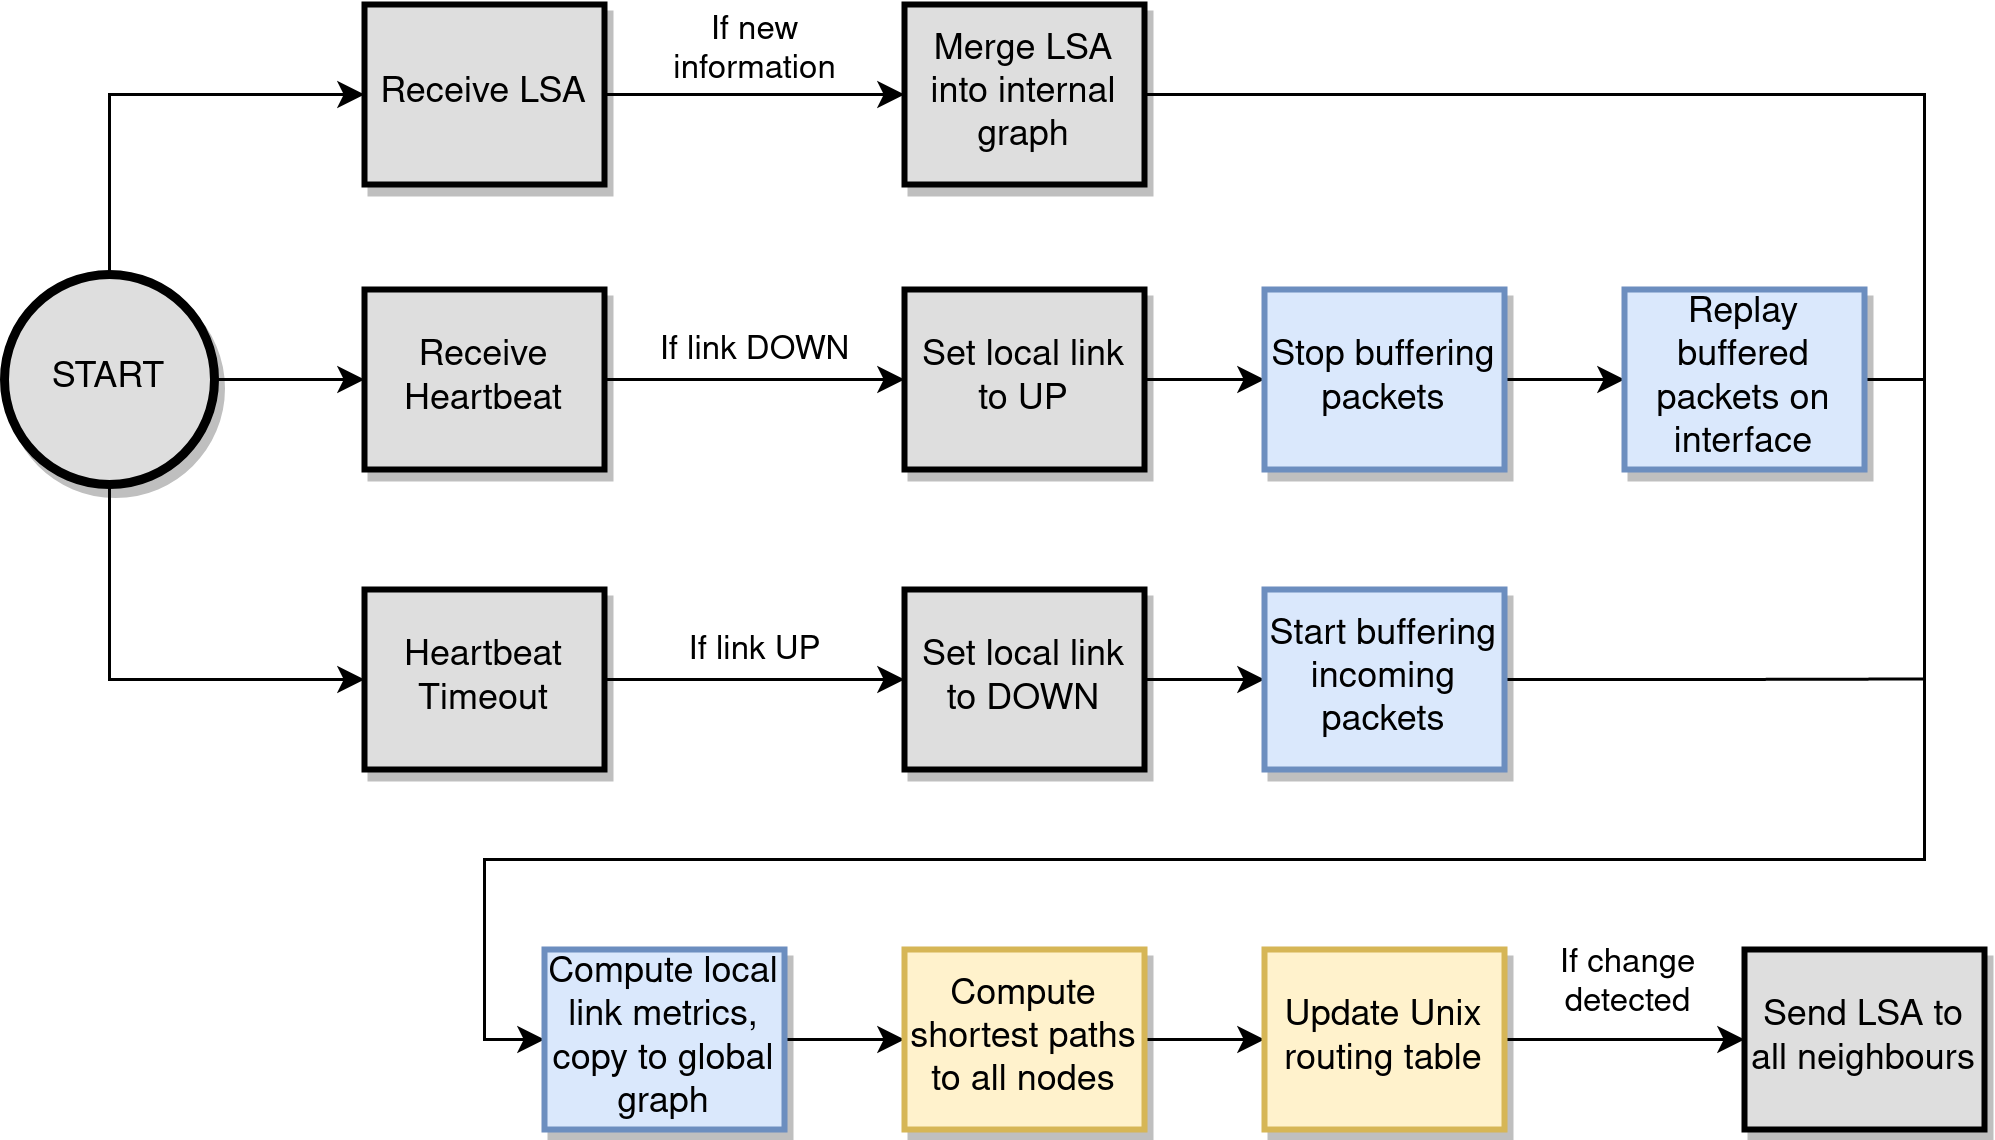
\includegraphics[width=1\textwidth]{flowchart_dtlsr}
	\captionof{figure}{Modified event loop of DTLSR}
	\label{fig:flowchart_dtlsr}
\end{minipage}
\end{center}

\begin{minipage}{1\textwidth} \centering
\begin{lstlisting}[language=C, label=preprocessor_switch, frame=tb, caption=Example of preprocessor switch for DTLSR modifications]
for (int i = 0; i < this->node.n_neighbours; i++) {
#ifdef DTLSR
  // For DTLSR, I use the more complex uptime metric
  this->node.link_metrics[i] =
      ts_compute_metric(&this->ls_time_series[i], now);
#else
  // For LSR, path cost is simply the hop count
  this->node.link_metrics[i] = 1.0;
#endif
}
\end{lstlisting}
\end{minipage}


\subsection{Packet Buffering}
\label{subsec:packet_buffering}

If an outgoing link from a router is down, in the delay-tolerant context the router is responsible for locally buffering incoming traffic that should be going out of the outgoing interface. This is done until either the link comes back up or a better alternative route appears, at which point it is sent on.

I use the \texttt{tcpdump} tool for interface listening. When a router knows a connected link is down, it starts listening on all interfaces and dumping received packets to a \texttt{pcap} file, according to a packet filter that only dumps packets going to IP addresses that are routed to via the down interface. Figure~\ref{fig:ip_route} shows an example of this, where the router buffers traffic en-route to the \texttt{10.0.2.0/24} or \texttt{10.0.3.0/24} subnets, as specified by the packet filter. Packets en-route to subnet \texttt{10.0.1.0/24} are forwarded like normal, without buffering.

\begin{figure}[H]
\centering
	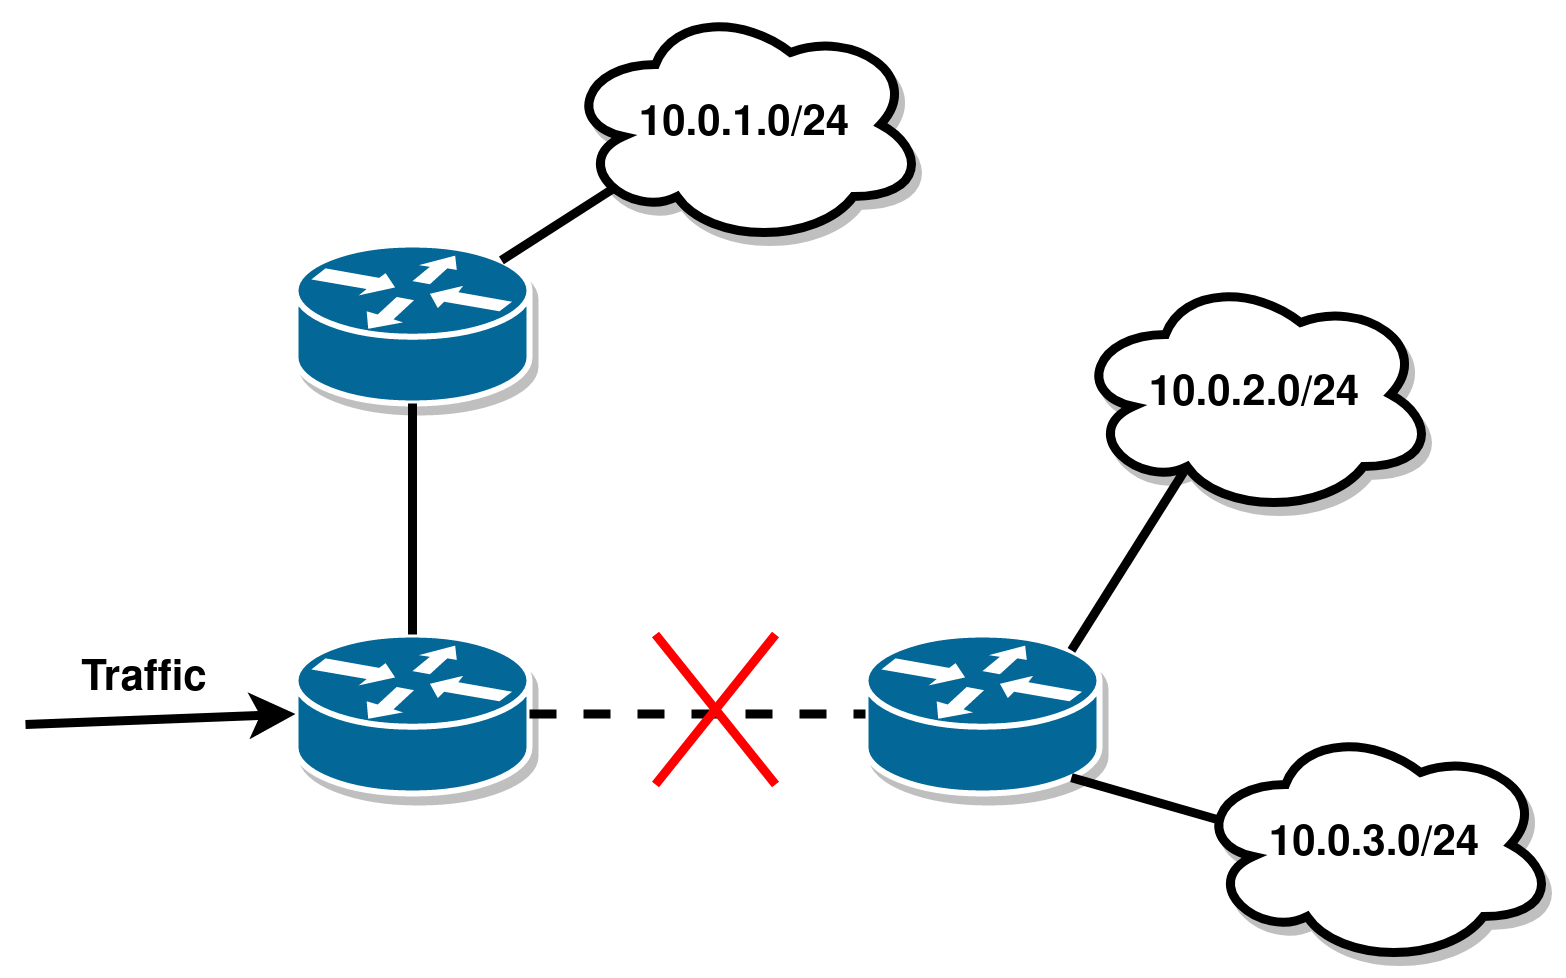
\includegraphics[width=0.54\textwidth]{ip_route}
	\captionof{figure}{Example of network that requires specific packet filtering}
	\label{fig:ip_route}
\end{figure}

I interact with \texttt{tcpdump} via the \texttt{libpcap} C library linked in statically with the executable, with the packet filter programmed using the Berkeley Packet Filter (BPF) language \cite{STEVEN1993}. An important optimisation is to place this \texttt{pcap} file on a RAM disk to maximise throughput and minimise latency that can occur when storing files on an SSD or HDD.

When the link comes back up, I stop listening for packets and dumping them to the file, and close the file. From now incoming packets are being sent onto the link correctly, so I don't want to duplicate data by buffering then resending it. I make use of a command-line tool, \texttt{tcpreplay}, which allows packets from \texttt{pcap} files to be replayed out of  an interface. We see the command-line call in Listing~\ref{replay_command}. I replay the packets, and then delete the file.

%Described here is the case of a single failing link, but when multiple links are concurrently failing and coming back up we of course need to be more careful about listening for and replaying only the right data.

\begin{lstlisting}[label=replay_command, caption=\texttt{tcpreplay} command with explanation of arguments, frame=tb]
tcpreplay --topspeed -ieth0 input.pcap

--topspeed - send packets as quickly as possible
-ieth0     - send on interface eth0
input.pcap - .pcap file to read packets from
\end{lstlisting}

I chose to use existing tools for packet buffering due to the complexity of this problem, as well as issues with reliability. Even a mature and tested tool like \texttt{tcpdump} still cannot catch all incoming packets at higher speeds; I would have no hope of implementing a suitable alternative in the time I had and it would likely be a part II project in its own right.

\subsection{Routing Through Down Links}
\label{subsec:routing_down_links}

In order for other nodes to send us their traffic to go through these down links, I must advertise routes as if the links were up. We take the first step in doing this by modifying the Dijkstra pathfinding algorithm to allow paths to go through DOWN links, which was prevented in the LSR protocol. With all of the paths generated, I proceed in the same way as the LSR protocol.

An interesting implementation detail is that I must add this route to the routers forwarding table. I must do this due to the feedback behaviour of ICMP: if a router receives a ping that must be forwarded on, but is not able to match its destination IP address in the forwarding table, then the kernel will drop the packet and send ICMP `\texttt{Network is unreachable}' response messages back to the sending source. The pings will still be buffered however, and once the link comes back up, they will be sent on to the actual destination which will send back to the source corresponding ping response messages. However the source will not accept these responses as they have already been nullified by the `\texttt{Network is unreachable}' messages, thus making ping unusable for evaluating the network. On the other hand, if I add the route to the forwarding table then these erroneous responses will not be generated by the router.

A downside to this is that incoming packets will be sent out of the interface onto the down link, deleting them. As I am buffering these packets as well, when the link comes back up there is a small chance of packet duplication, however for testing purposes this is not an issue. To resolve this in a full implementation one would have to modify the behaviour of ICMP in the kernel, as well as potentially other network-layer protocols that have similar behaviour. I wanted to remain in userspace for ease of implementation, so as it has no effect on my evaluation I left it be.

\subsection{Link Metric}
\label{subsec:link_metric}

I need some metric to be able to judge the expected delay of a link, in order to compare it to a stable backup link that I can switch onto when appropriate, to minimise the overall delay. This alternative metric is needed only when the link is down, as this is the case when I would want to switch. When the link comes back up it is desirable to send out the buffered packets as quickly as possible, so a metric with some level of hysteresis as described below is inappropriate. Through testing, it is far more effective to immediately fall back to the standard hop-count metric once the link comes back up.

Assuming that the link will come back up, not switching to the backup link will have no effect on delivery rate as the packets will be buffered, and will reach their destination eventually. However doing this increases the average delay that packets experience, as waiting for the link to come back up will take longer than simply sending via the backup route. Some level of hysteresis for this is beneficial so that if failures are historically rare and short-lived, the router sticks to the primary link.

I use a metric based on the uptime history of the link, computing an integral over the history after exponentially weighting it, as seen in Figure~\ref{fig:metric}. Integrating over the uptime history describes how often the link is up, giving some idea of its reliability over time, and the exponential weighting gives more importance to recent events, making it more responsive.

Equation~\ref{eq:metric_integral} shows how I compute the integral over one UP period, between times $t_0$ and $t_1$. The falloff parameter $\alpha$ tunes the metrics responsiveness to changing conditions, increasing it increases the falloff. I compute this integral over each of the UP periods, summing the results together in Equation~\ref{eq:metric_sum} to give $F$.

\begin{equation} \label{eq:metric_integral}
F(t_0, t_1) = \int_{t_0}^{t_1} f(t)dt = e^{\alpha \cdot t_1} - e^{\alpha \cdot t_0}
\end{equation}

\begin{equation} \label{eq:metric_sum}
F = \sum_{i = 0}^{|\textbf{History}|/2} F(t_{2i}, t_{2i+1})
\end{equation}

\begin{equation} \label{eq:metric_final}
\textit{metric} = \Big\lfloor\frac{1}{F+0.00002}\Big\rfloor
\end{equation}

The value of $F$ decreases approaching zero as the uptime decreases approaching zero, but I choose to inverse this relationship as routes with lower value metrics are chosen with higher preference. As uptime approaches zero, the metric should increase approaching some large value. In the Unix routing table metrics are stored as a 16-bit unsigned integer, which has a maximum value of 65,535. The maximum value of the metric should be bounded below this to prevent integer underflow, which would assign the wrong metric to the route. The final metric is that shown in Equation~\ref{eq:metric_final}, which has a maximum value of 50,000 when $F$ is 0. Furthermore, when the uptime is 100\% the metric takes its minimum value of 1, equal to the hop count of a single UP link that is used in LSR.

\begin{center}
\begin{minipage}{0.9\textwidth} \centering
	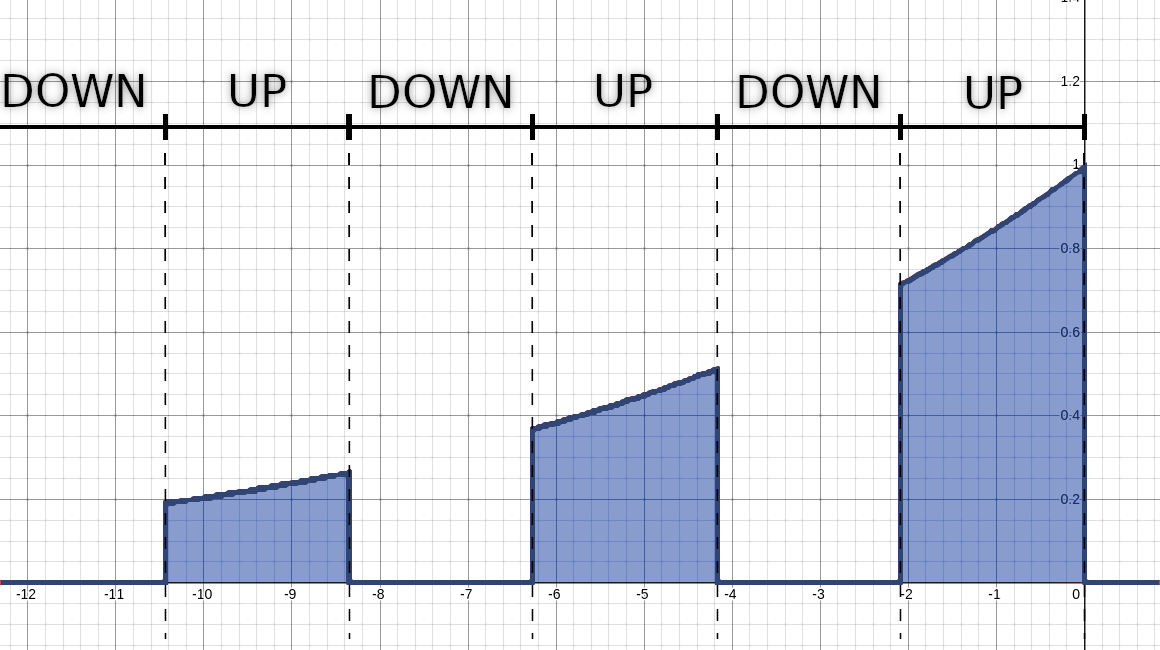
\includegraphics[width=0.9\textwidth]{metric}
	\captionof{figure}{Diagram showing the exponentially weighted integral that gives $F$}
	\label{fig:metric}
\end{minipage}
\end{center}

I store the uptime history as a circular array of Unix timestamps, each representing the time of an UP or DOWN event. As I know the current state of the link, I can work my way backwards through the array to compute which type of event any given timestamp represents, rather than explicitly storing it. Once the array fills up I start overwriting old events to save memory, however discarding these values has negligible effect on the metric due to the exponential weighting.

The timestamps signify the times of events, but I calculate the metric with respect to the current time. If the last event was a DOWN event, we can imagine the function plot in Figure~\ref{fig:metric} sliding left, changing the value of the metric over time due to the exponential weighting. Because of this changing metric I must periodically update the routing table, as there may be alternative routes with a lower path cost due to the metric increasing.

\section{Implementation Practicalities}

Some parts of the implementation were hard-coded or have inefficient solutions to aid in creating a functional piece of software that could be evaluated more quickly. These are sections that have no impact on the evaluation of the protocol as a solution to the routing problem, or are even completely unrelated to routing in general.

As an example I ran into the issue of \textit{neighbour discovery}, where nodes generally use the link-level ARP protocol to discover the existence of neighbouring nodes on their interfaces. The ARP table in CORE proved unreliable, and as this is a link-layer problem unrelated to routing I simply hardcoded all immediate neighbours in configuration files. Implementing actual neighbour discovery would provide no practical benefits to the evaluation, and could even negatively impact it if my implementation was unreliable or had varying performance.

An example of hardcoding is that the memory representation of the link-state graph is statically allocated, i.e.\ the maximum number of nodes in the network is specified as a compile-time constant. The advantage of this is that it makes indexing and bounds checking very easy and computationally efficient. However, this has the twin disadvantages of wasting memory if the number of nodes is below the maximum and, much worse, crashing if the number of nodes increases beyond the maximum. For the evaluation, this is not an issue, as I know beforehand the size and topology of all networks being tested and can adapt the compile-time maximum as needed. If used in a real, dynamic network, the memory representation would have to be changed to allow dynamic sizing.

While CORE supports IPv6 addressing, I restricted myself to only supporting IPv4 to reduce the unnecessary complexity of supporting another addressing scheme that would have no impact on the performance of the routing protocol, and thus not help my evaluation at all.

\section{Repository Overview}

\begin{minipage}{1\textwidth} \centering
\begin{lstlisting}[label=repository, frame=tb]
dtlsr                        Root
|- configs                   CORE config files
|- include                   Include directory
|  |- algorithm
|  |- network
|  +- process
|- src                       Source directory
|  |- algorithm
|  |- network
|  +- process
|- tests                     Unit tests directory
|  |- algorithm
|  |- network
|  +- process
|- tools                     Custom development tools
+- core-py                   Custom CORE scripts
\end{lstlisting}
\end{minipage}

\begin{itemize}
	\item
	\texttt{algorithm} contains pure algorithms and data structures, for example the graph representation, pathfinding, and heap implementations.

	\item
	\texttt{network} contains functionality for socket manipulation, sending data over the network, and packet listening/replay.
	
	\item
	\texttt{process} contains functionality for interacting with both CORE and the Unix OS, for example retrieving node information, logging, and manipulating the Unix routing table.
\end{itemize}

The project was implemented almost entirely in C, with CORE-specific scripts in Python.

\subsection{Repository Justification}

The \texttt{src/}, \texttt{include/}, and \texttt{tests/} directory separate code from the build system, as well as being separated from each other as they each serve a different purpose. Within these folders sources files are separated by purpose as described above, with the groupings being important to encourage good header inclusion practice, reducing the complexity of programming in the long run.


\chapter{Evaluation}
\label{chapter:evaluation}

I perform the evaluation using the CORE emulator. I define a network topology of hosts and routers, with the routers running either the LSR or DTLSR routing protocol, to compare the performance of both for a variety of metrics on a variety of different topologies.

\paragraph{Convergence}
I first determine the convergence behaviour of the protocols to provide a baseline of the testing environment. I do this with LSR, but as DTLSR's system for LSA sharing is identical, the results are valid for both. Convergence time is essential for a discussion of delay, as included in the delay is the time taken for routers to respond to changes in the network state; minimising the convergence time should aid us in minimising overall packet delay.


\paragraph{Delay and Delivery Rate}
I then compare the delay of packet arrivals in LSR and DTLSR in a number of topologies, importantly providing the overall packet loss percentage as well. Packet loss has a critical influence on delay, as the time taken to detect a loss and retransmit can be many orders of magnitude above the time to propagate a packet through the network, drastically increasing the mean delay. It is necessary to also consider that information may be spread across multiple packets, meaning that individual packet losses can prevent us from using already received data that depends on it, causing a bottleneck. Thus, minimising packet drop rate is critically important.

\paragraph{TCP Throughput}
I then briefly evaluate TCP's throughput performance on an unreliable network, seeing how link flapping exposes fundamental problems with TCP's rate control feedback mechanism. While not the main focus of this project, this gives us some insight into the larger-scale issues of implementing a delay-tolerant network stack in the real world.


\section{Convergence}

The convergence time of the link-state protocol, is the time between the state of the graph updating (e.g.\ a link going down), and that change being detected and incorporated into the routing table of a particular node in the network. As changes are propagated from node-to-node, I expect that convergence time increases as the node's distance from the changing link increases. I will distinguish the convergence time in response to links going down, and links coming back up, as these are detected in different ways. 

My testing topology is a long chain of routers, shown in Figure~\ref{fig:conv_topology}, with the flapping link \texttt{n1-n2} on the far left end and the update messages being propagated down the chain. This gives me a way to detect how long it takes a node to detect the change for each number of router `hops'.

\begin{minipage}{1\textwidth} \centering
	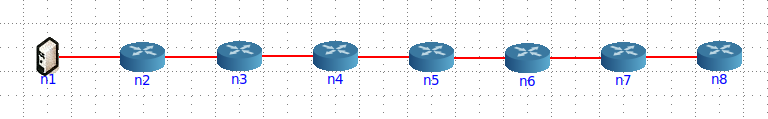
\includegraphics[width=0.9\textwidth]{conv_topology}
	\captionof{figure}{`Convergence' network topology}
	\label{fig:conv_topology}
\end{minipage}

I flap the link using the Python scripting API that CORE provides, waiting 4 seconds between each state change---long enough that it guarantees that all nodes have fully converged before I modify the state again. I log the time when this occurs.

I monitor each node's routing table using the \texttt{route} Unix utility, the output of which is shown in Listing~\ref{route_command}, with a simple Python script that logs the time when I detect that the route corresponding to node \texttt{n1} has either appeared or disappeared from the table, respective to the link being up or down. I then analyse the data to determine the time between the link changing state, and each node detecting this change and modifying its routing table accordingly.

\begin{lstlisting}[label=route_command, caption=Example routing table of virtualised node, frame=tb]
ben@ben-laptop:~/dtlsr/tools$ python3 vcmd.py n5 route -n
Kernel IP routing table
Destination Gateway  Genmask       Flags Metric Ref Use Iface
10.0.0.0    10.0.0.6 255.255.255.0 UG    1      0     0 eth0
10.0.1.0    10.0.4.4 255.255.255.0 UG    2      0     0 eth1
10.0.2.0    10.0.4.4 255.255.255.0 UG    3      0     0 eth1
10.0.3.0    10.0.0.6 255.255.255.0 UG    2      0     0 eth0
...       
\end{lstlisting}

I do convergence testing with link delays of \SI{1}{\ms} and \SI{100}{\ms}. A link delay of \SI{100}{\ms} is large enough to verify that the convergence time depends on the hop count, from the propagation time, while a delay of \SI{1}{\ms} is what I use for the rest of the evaluation, so it is useful to include as a baseline.  Heartbeats are sent every \SI{200}{\ms}, and the heartbeat timeout is set to \SI{900}{\ms}.

\begin{minipage}{1\textwidth}
\subsection{Results}

The graphs in Figure~\ref{fig:conv} show the time between the event occurring and it being detected by the router, depending on the number of hops from the event. Error bars are the standard deviation of the convergence time. I consider the zero-hop node to be that directly attached to the flapping link. Figures~\ref{fig:conv_1ms} and \ref{fig:conv_100ms} both show a marked difference between the detection time of the UP and DOWN events, where detection of the link coming up happens much faster than detecting it has failed. This is due to the way these are detected at a link-level, with the former being actively detected by a heartbeat and the latter being passively detected by a timeout. It is then clear that these rely heavily on the particular constants chosen for the heartbeat sending period and the amount of time required for a timeout.

\begin{figure}[H]
\centering
\begin{subfigure}{.5\textwidth}
  \centering
  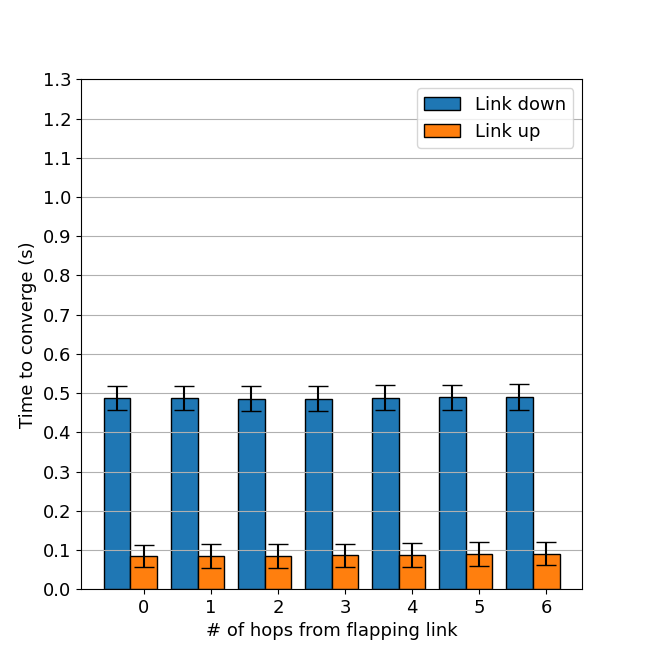
\includegraphics[width=1\linewidth]{conv_1ms}
  \caption{Link delay of \SI{1}{\ms}}
  \label{fig:conv_1ms}
\end{subfigure}%
\begin{subfigure}{.5\textwidth}
  \centering
  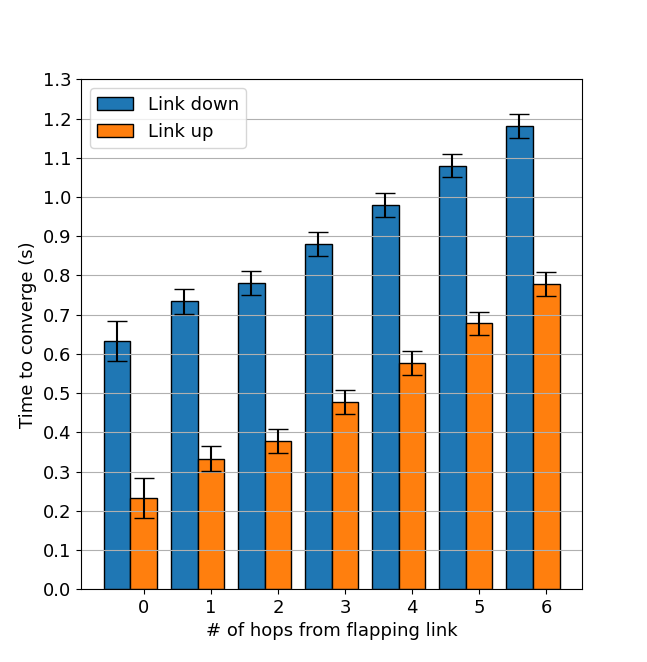
\includegraphics[width=1\linewidth]{conv_100ms}
  \caption{Link delay of \SI{100}{\ms}}
  \label{fig:conv_100ms}
\end{subfigure}
\caption{Protocol convergence times against hop count}
\label{fig:conv}
\end{figure}

\end{minipage}

Hop counts of 1 and above rely on the network-layer section of the protocol, with link-state information being sent from node to node. As rLSAs are propagated almost as soon as they are received, convergence time is bounded mainly by the link delay, which we can see in the difference between the higher hop counts of~\ref{fig:conv_1ms} and~\ref{fig:conv_100ms}. In~\ref{fig:conv_1ms} the delay is so small as for each subsequent hop to be almost indistinguishable from the last, but Figure~\ref{fig:conv_100ms} shows the delay increasing the convergence time for each hop cumulatively, for both UP and DOWN events.

It is interesting to note that subsequent hops depend on the cumulative time added by all previous hops, due to propagation. As the difference between up and down remains close to constant after the zero-hop node, I conclude that the network-layer behaviour is the same for up and down, explained by them both depending on the same rLSA propagation system.


\section{Delay: Link Failures}

The main body of the evaluation compares the distribution of round-trip packet delays for LSR and DTLSR in a number of different network environments with varying topologies and failure modes. This demonstrates the different properties of the routing algorithms, showing the advantages and disadvantages of both.

I evaluate with UDP to minimise any interference the transport layer may have on testing. I approximate UDP with the Unix \texttt{ping} utility, which, despite using ICMP, emulates the behaviour of UDP well at higher throughputs, similarly having no flow and congestion control mechanisms. I take the `delay' of a packet as being the round-trip time as computed by \texttt{ping}.

I plot the distribution of delays as a logarithmic CDF plot with the y-axis signifying the proportion of packets, with an example shown in Figure~\ref{fig:partition}. When the line goes off the edge of the graph on the right without reaching 1.0 on the y-axis, it shows that the remaining proportion of packets was dropped. I do not include retransmissions as this is a transport-layer responsibility.

Unless specified otherwise, all links have a delay of \SI{1}{\ms}.

\subsection{Partial Partition Topology}
\label{subsec:partial_partition}

Firstly, I use a topology with a single central connecting link, \texttt{n1-n2}, that I periodically alternate being up or down; we say that the link is \textit{flapping}. Of note in this topology is that when the link is down it creates a network partition between node subsets \texttt{(n1,n3,n5)} and \texttt{(n2,n4,n6)}.

\begin{minipage}{1\textwidth} \centering
	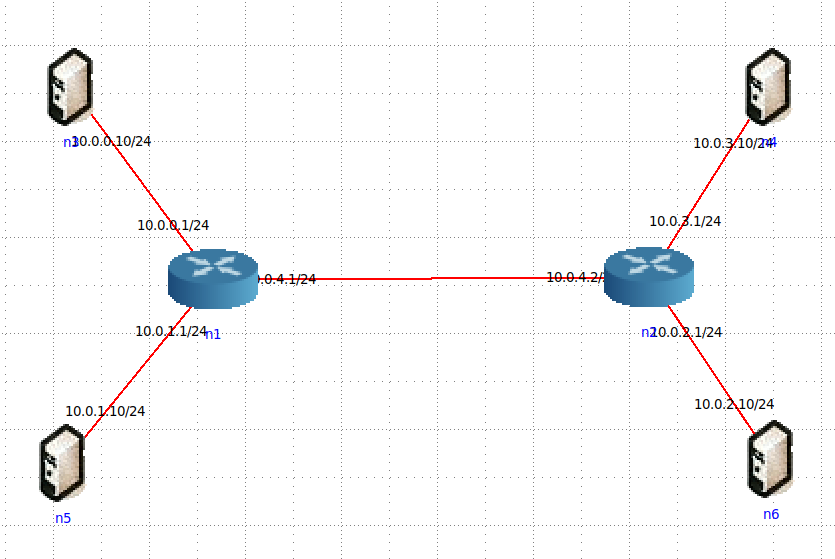
\includegraphics[width=0.5\textwidth]{delay_partition_topology}
	\captionof{figure}{\textbf{Partial partition} network topology.}
	\label{fig:partition_topology}
\end{minipage}

The results are shown in Figure~\ref{fig:partition} as cumulative distributions of round-trip delay between \texttt{n5} and \texttt{n6} under different routing algorithms while flapping link \texttt{n1-n2}. In both cases LSR successfully delivers a proportion of packets approximately the same as that of the uptime proportion of the link, in Figure~\ref{fig:partition_20} it is up half of the time, so there is 50\% delivery, and in Figure~\ref{fig:partition_2_18} it is up one tenth of the time, so there is a 10\% delivery rate. DTLSR achieves a drastically higher delivery ratio in both cases due to packets being buffered at the router before the failure, then forwarded on when it comes back up.

\begin{figure}[h]
\centering
\begin{subfigure}{.5\textwidth}
  %\centering
  %\hspace*{1.1cm}
  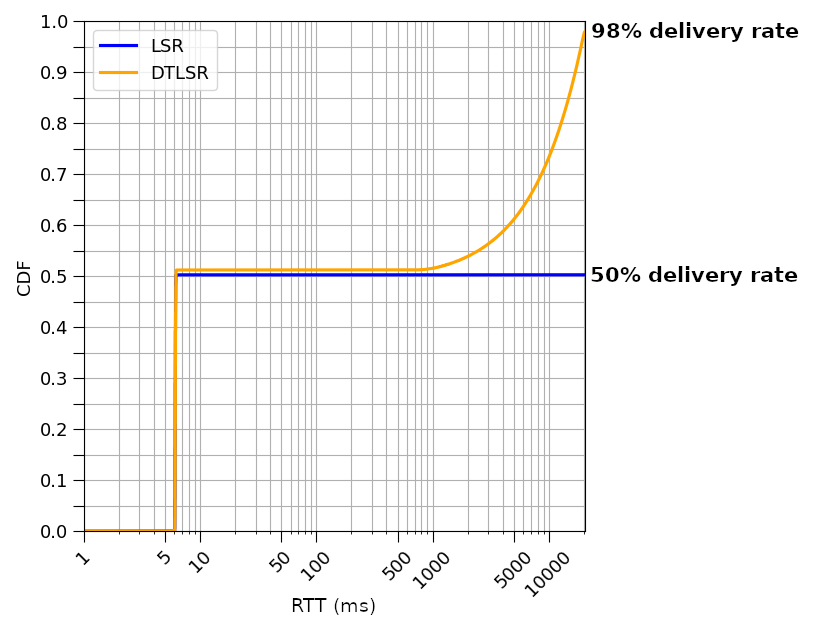
\includegraphics[width=1\linewidth]{delay_partition_flap20}
  \caption{Flapping period $T=\SI{40}{\s}$ (\SI{20}{\s} up, \SI{20}{\s} down)}
  \label{fig:partition_20}
\end{subfigure}%
\begin{subfigure}{.5\textwidth}
  %\centering
  %\hspace*{1.1cm}
  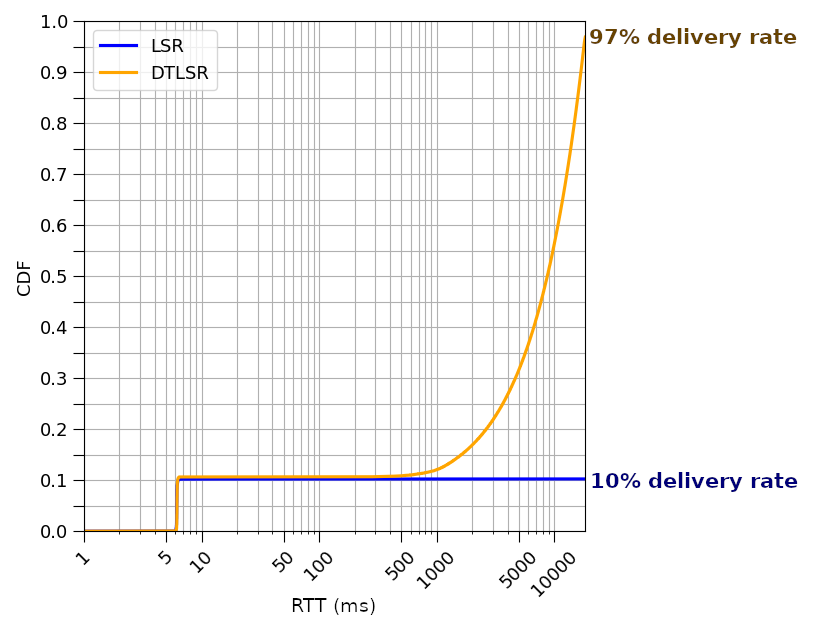
\includegraphics[width=1\linewidth]{delay_partition_flap2_18}
  \caption{Flapping period $T=\SI{20}{\s}$ (\SI{2}{\s} up, \SI{18}{\s} down)}
  \label{fig:partition_2_18}
\end{subfigure}
\caption{Cumulative distributions of round-trip delay showing overall packet delivery rates}
\label{fig:partition}
\end{figure}

In both plots the packets can be split into two groups. For the first group both LSR and DTLSR have a constant delay of \SI{6}{\ms}. For LSR the second group of packets are dropped, whereas for DTLSR their delay increases linearly (showing as an exponential curve in the $\log x$-$y$ graph). The first group is due to the link being up the described proportion of the time of the time, so all packets sent in this period take approximately the same time to arrive, taking a round-trip journey over three links (\texttt{n5-n1-n2-n6}) each of \SI{1}{\ms} delay. The second group is a little more subtle, and is due to the packet buffering and replaying behaviour. \texttt{ping} sends packets at a constant interval but the buffered packets are replayed all at once when the link comes back up, thus the earlier that a ping is sent in the link-down period, the greater time delay there will be between the client sending the packet and receiving a reply. The annotated \texttt{ping} trace in Listing~\ref{ping_trace} shows an example with the packet's round-trip-times and sequence numbers, responding to a link that is down for three seconds.

\begin{lstlisting}[label=ping_trace, caption=Example \texttt{ping} trace with link flapping, frame=tb]
[...] 10.0.2.3: icmp_seq=4 ttl=62 time=6.20 ms
[...] 10.0.2.3: icmp_seq=5 ttl=62 time=6.05 ms
[...] 10.0.2.3: icmp_seq=6 ttl=62 time=6.20 ms
[...] 10.0.2.3: icmp_seq=7 ttl=62 time=3272 ms <- link down
[...] 10.0.2.3: icmp_seq=8 ttl=62 time=2872 ms
[...] 10.0.2.3: icmp_seq=9 ttl=62 time=2441 ms
[...] 10.0.2.3: icmp_seq=10 ttl=62 time=2025 ms
[...] 10.0.2.3: icmp_seq=11 ttl=62 time=1609 ms
[...] 10.0.2.3: icmp_seq=12 ttl=62 time=1193 ms
[...] 10.0.2.3: icmp_seq=13 ttl=62 time=777 ms
[...] 10.0.2.3: icmp_seq=15 ttl=62 time=6.29 ms <- link up
[...] 10.0.2.3: icmp_seq=16 ttl=62 time=6.06 ms
[...] 10.0.2.3: icmp_seq=17 ttl=62 time=6.18 ms
\end{lstlisting}

This variability in delay can be undesirable, but it is not something that can be fixed as partitioning is a fundamental property of the network that can't be worked around. Even a perfect retransmission protocol would run into the same variability issue, retransmitting all of the dropped packets as soon as the link came back up. Users of the network should take this into account with the applications that they decide to run on it, and ensure that there are not strict low-latency requirements with applications like video conferencing or real-time games.

A comparison of Figures~\ref{fig:partition_5} and \ref{fig:partition_20} shows that increasing the flapping frequency creates a higher drop rate overall for both protocols, which can be explained by considering that when a link goes down it takes time for the router to detect this change, in which time any incoming packets are sent out of the interface and are summarily deleted. It is only once the state change is detected that the protocol changes the routing table or starts buffering packets, for LSR and DTLSR respectively. The higher the flapping frequency, the higher proportion of time is spent spend in these `boundary' periods, and thus the more packets both LSR and DTLSR drop.

\begin{figure}[h]
  \centering
  %\hspace*{2.4cm}
  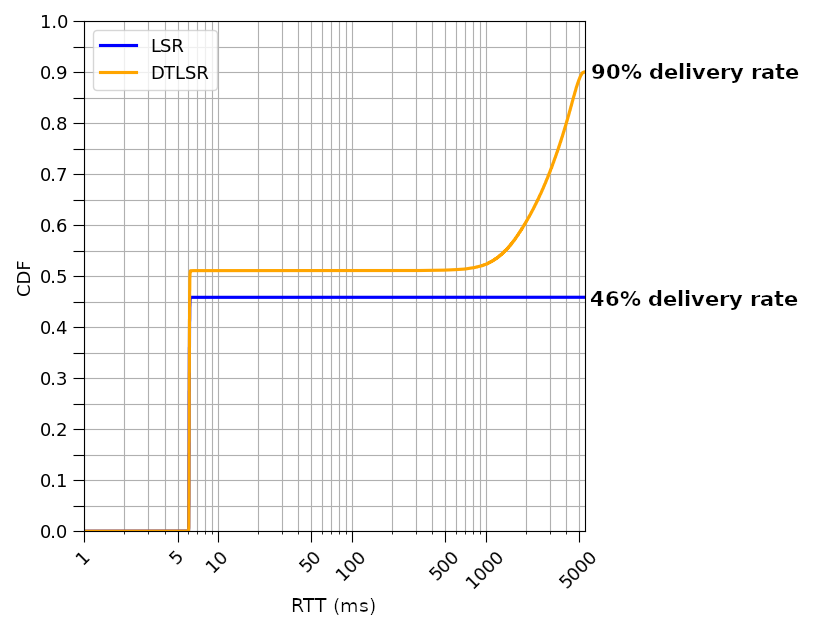
\includegraphics[width=0.5\linewidth]{delay_partition_flap5}
  \caption{Flapping with period $T=\SI{10}{\s}$ (\SI{5}{\s} up, \SI{5}{\s} down).}
  \label{fig:partition_5}
\end{figure}

This network topology is consistent with those seen in remote regions even in developed countries, where there is a single main link being relied on. If that link becomes unreliable, then I have shown that using a delay-tolerant routing protocol greatly increases the proportion of packets delivered. As the proportion of time the link spends up decreases, the advantage in packet delivery that DTLSR has over LSR increases drastically.


\subsection{Full Partition Topology}

The second topology shown in Figure~\ref{fig:full_partition_topology} is similar to the above \textbf{Partial partition} topology, but instead partitions the network with two links in sequence that have anti-correlated failures as shown in Figure~\ref{fig:full_partition_graph}---when one is up, the other is down. Thus, there is never any end-to-end connection and the network is technically always partitioned, but using the \textit{store-and-forward} mechanism some packet delivery can be achieved. This is not as ridiculous a case as it may seem: if a region has unreliable or limited power, there may only be sufficient power to turn on a subset of the routers at a time, likely in an unpredictable pattern.

\begin{figure}[H]
\centering
\begin{subfigure}{.65\textwidth}
  \centering
  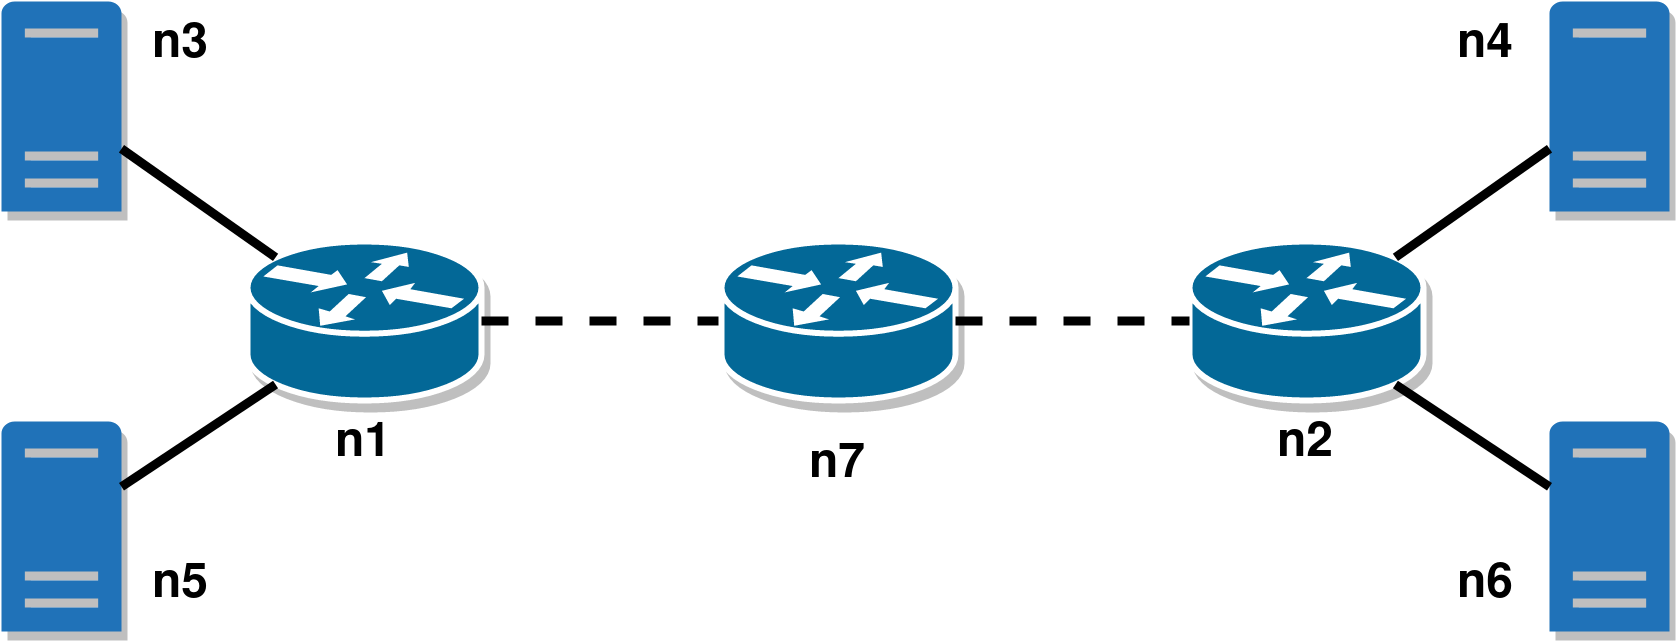
\includegraphics[width=1\linewidth]{delay_full_partition_topology}
  \caption{}
  \label{fig:full_partition_topology}
\end{subfigure}

\begin{subfigure}{.65\textwidth}
  \centering
  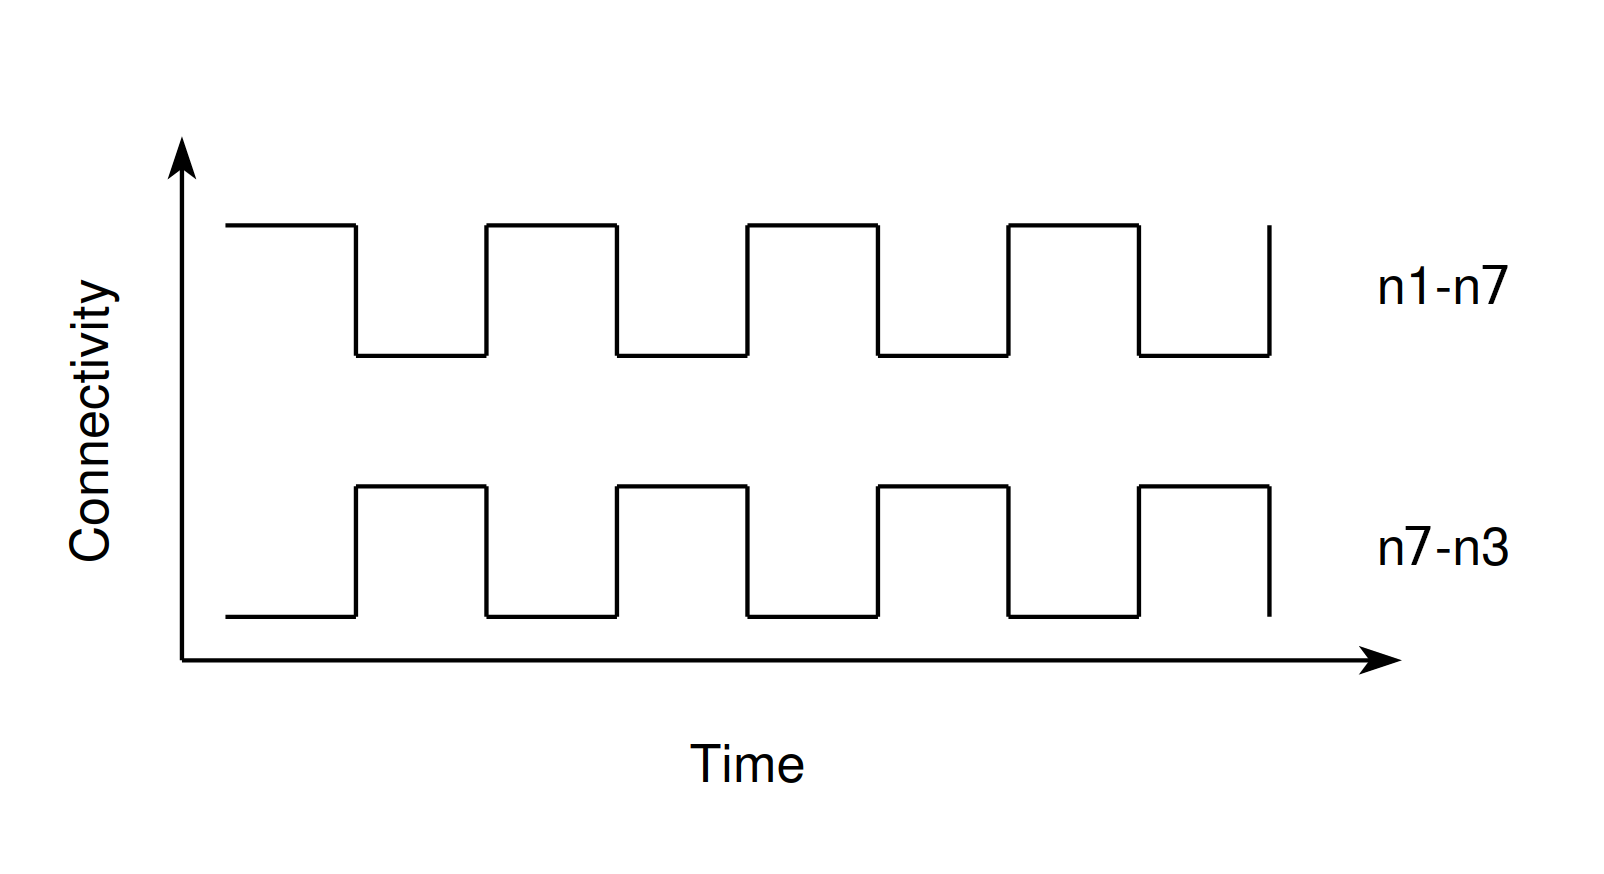
\includegraphics[width=1\linewidth]{delay_full_partition_graph}
  \caption{}
  \label{fig:full_partition_graph}
\end{subfigure}
\caption{\textbf{Full partition} network topology with anti-correlated link failures.}
\label{fig:full_partition}
\end{figure}

Figure~\ref{fig:full_partition_flap} shows that LSR achieves zero packet delivery, compared to DTLSR achieving upwards of 70\% percent overall. This is notably much more serious than the results above, where LSR achieved a lower but still greater-than-zero delivery, as retransmission-based transport protocols rely on the fact that there is \textit{some} packet delivery, where in the limit of time with retransmissions the probability of delivery approaches 1. However with zero delivery, this limit stays at zero and thus the unreliable network cannot be made reliable with a transport layer protocol. Achieving any communication whatsoever relies entirely on the routing layer's packet buffering system.

As the flapping period increases, reducing the frequency of boundary events, a comparison of Figures~\ref{fig:full_partition_flap5} and \ref{fig:full_partition_flap20} again show that the packet delivery rate increases. However it is not as large of an increase as seen in the other topologies.

\begin{figure}[H]
\centering
\begin{subfigure}{.5\textwidth}
  %\centering
  %\hspace*{1.1cm}
  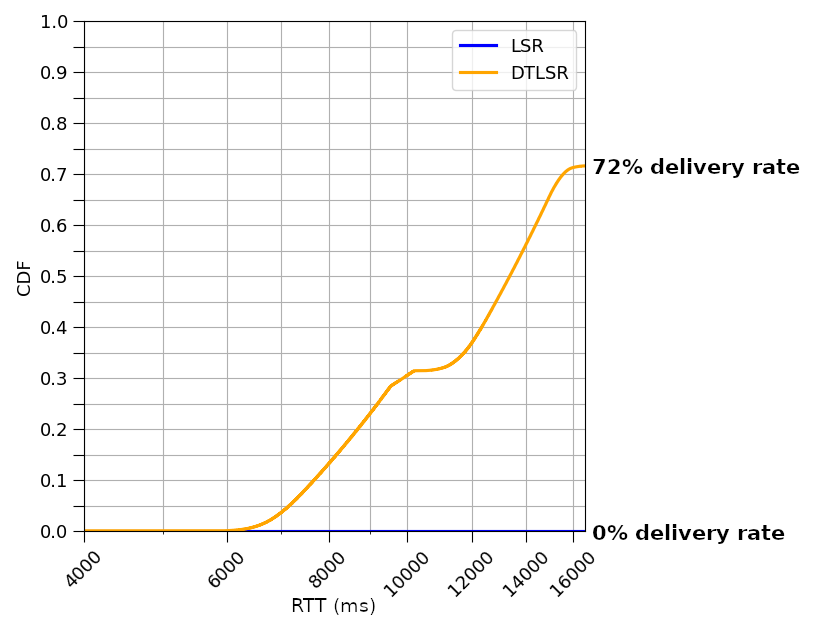
\includegraphics[width=1\linewidth]{delay_full_partition_flap5}
  \caption{Flapping period $T=\SI{10}{\s}$ (\SI{5}{\s} up, \SI{5}{\s} down)}
  \label{fig:full_partition_flap5}
\end{subfigure}%
\begin{subfigure}{.5\textwidth}
  %\centering
  %\hspace*{1.1cm}
  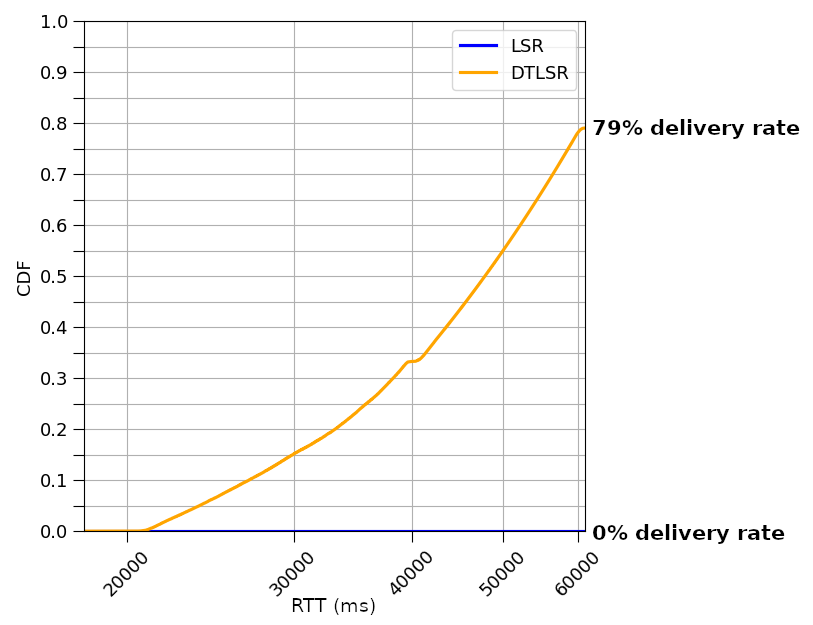
\includegraphics[width=1\linewidth]{delay_full_partition_flap20}
  \caption{Flapping period $T=\SI{40}{\s}$ (\SI{20}{\s} up, \SI{20}{\s} down)}
  \label{fig:full_partition_flap20}
\end{subfigure}
\caption{Cumulative distributions of round-trip delay showing overall packet delivery rates}
\label{fig:full_partition_flap}
\end{figure}

It's interesting to note that increasing the flapping period causes an approximately proportional increase in the packet delay, with packets having a delay around four times as large with $T=40$ than $T=10$. This is because packets are spending the vast majority of their time waiting for the link to come back up. It is a similar phenomenon to driving down a long road with traffic lights in series; if the lights are anti-correlated then you will be stopped at each in turn, and your progress down the road will depend almost entirely on the switching frequency of the lights.


\subsection{Box Topology}

The third topology shown in Figure~\ref{fig:box} is a `box'-shaped one, where there is a low-delay main route and a higher delay backup route when the main one goes down. In this example \texttt{n3-n4} is the flapping main link, and \texttt{n3-n5-n6-n4} is the higher-delay backup route. The backup link \texttt{n5-n6} has a delay of \SI{10}{\ms}, and as usual all other links have a delay of \SI{1}{\ms}. Thus from \texttt{n1} to \texttt{n2}, the main route has a round-trip delay of \SI{6}{\ms} and the backup route has a round-trip delay of \SI{28}{\ms}.

\begin{figure}[h]
\centering
	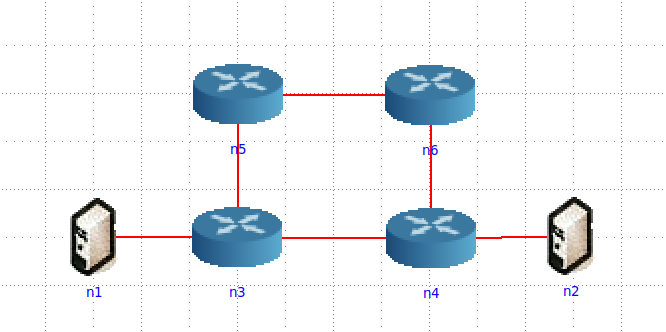
\includegraphics[width=0.6\textwidth]{delay_box_topology}
	\captionof{figure}{\textbf{Box} network topology.}
\end{figure}

Both cases of Figure~\ref{fig:box} show that LSR successfully switches to the backup link whenever the main link goes down, shown by a large proportion of packets having an RTT of approximately \SI{28}{\ms}. As described above, it takes time for the protocol to detect that the link is down and to respond by modifying the routing table, which causes packet losses. Increasing the flapping frequency increases the number of these boundary periods, thus increasing the proportion of time dropping packets. This is reflected in the higher proportion of packets being dropped with a shorter flapping period for LSR in Figure~\ref{fig:box_2}.

\begin{figure}[h]
\centering
\begin{subfigure}{0.5\textwidth}
  %\centering
  %\hspace*{1.1cm}
  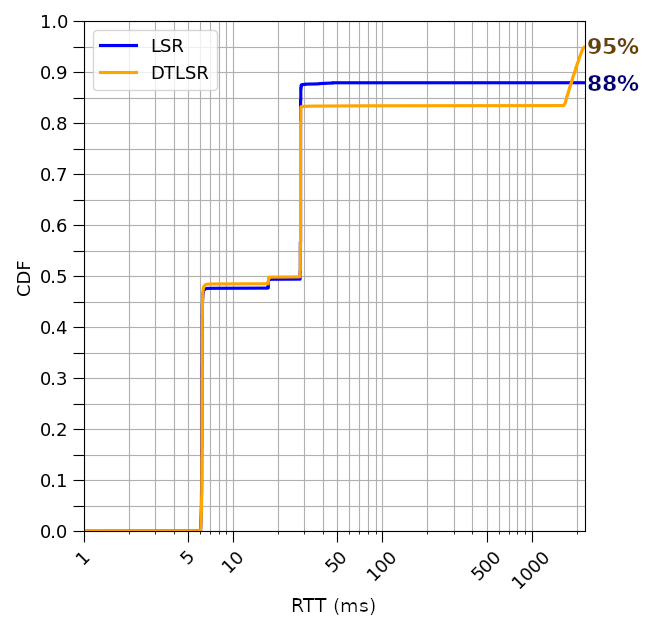
\includegraphics[width=1\linewidth]{delay_box_flap2}
  \caption{Flapping period $T=\SI{4}{\s}$ (\SI{2}{\s} up, \SI{2}{\s} down)}
  \label{fig:box_2}
\end{subfigure}%
\begin{subfigure}{0.5\textwidth}
  %\centering
  %\hspace*{1.1cm}
  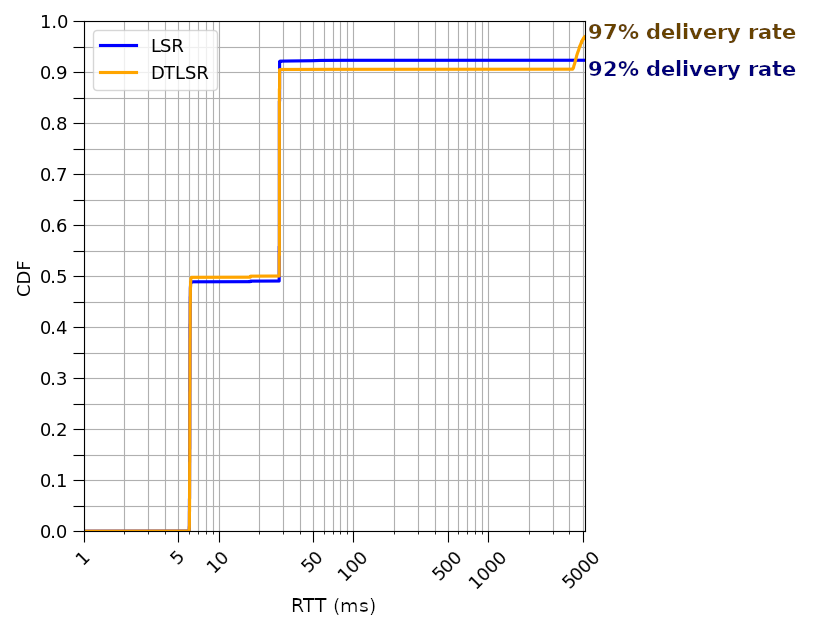
\includegraphics[width=1\linewidth]{delay_box_flap5}
  \caption{Flapping period $T=\SI{10}{\s}$ (\SI{5}{\s} up, \SI{5}{\s} down)}
  \label{fig:box_5}
\end{subfigure}
\caption{Cumulative distributions of round-trip delay showing packet delivery rates}
\label{fig:box}
\end{figure}

Figure~\ref{fig:box} again shows that DTLSR achieves a higher proportion of delivered packets than LSR. While it is a lot closer than in the partition topology, there is still a marked difference. DTLSR uses its metric to judge the failed link in comparison to the backup link, switching onto it shown by DTLSR also having a large portion of packets having a delay of around \SI{28}{\ms}. DTLSR is slightly slower to switch the route due to the metric's hysteresis, shown by LSR having a slightly higher proportion of packets with \SI{28}{\ms}. However DTLSR ends up with a higher delivery rate overall due to the packet buffering, shown on the top right of each of the graphs.

As stated above this kind of topology is uncommon in remote and developing regions due to the cost of adding backup links. However it is useful to contrast LSR and DTLSR and show that even with other hardware solutions to failure, DTLSR still has a competitive advantage over LSR in delivery rate.

\section{Delay: Node Failures}

As detailed in section~\ref{sec:link_vs_node_failures}, considering the effects of router failures on the delay of packets through the network is necessary, as their recovery process is a little different to link failures. I evaluate using the topology described in Figure~\ref{fig:node_partition_topology}, periodically shutting down and restarting the node \texttt{n7} with period $T=40$ (\SI{20}{\s} up, \SI{20}{\s} down). When the node is down the network is partitioned, similarly to the \textbf{Partial partition} topology in section~\ref{subsec:partial_partition}.

\begin{figure}[H]
  \centering
  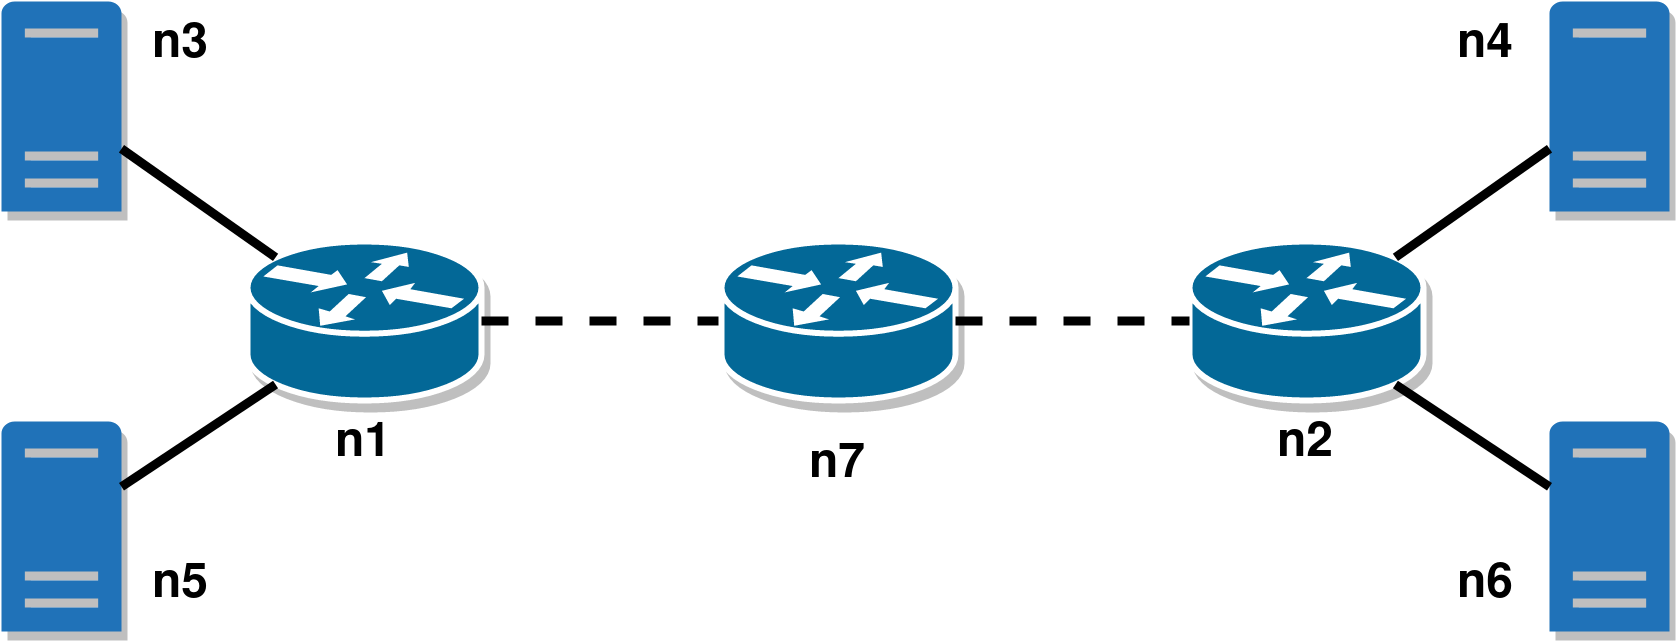
\includegraphics[width=0.65\linewidth]{delay_full_partition_topology}
  \caption{\textbf{Node} partition topology}
  \label{fig:node_partition_topology}
\end{figure}

\subsection{Results}

Figure~\ref{fig:delay_node_flap20} shows identical behaviour to the results of link failure in Figure~\ref{fig:partition_20}, with LSR achieving 50\% delivery rate consistent with the router being up half of the time, and DTLSR achieving a much higher 98\% delivery rate due to the packet buffering at \texttt{n1} and \texttt{n2}. The 2\% packet loss is again due to \texttt{n1} and \texttt{n2} only detecting the down node after the heartbeat timeout period.

\begin{figure}[h]
	\centering
	%\hspace*{2.4cm}
	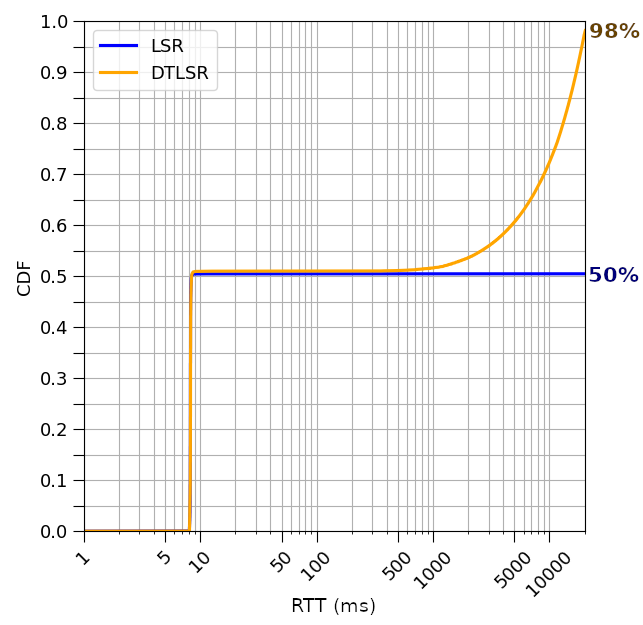
\includegraphics[width=0.5\textwidth]{delay_node_flap20}
	\captionof{figure}{CDF of packet round-trip delay for node-failure topology}
	\label{fig:delay_node_flap20}
\end{figure}

That node failure under DTLSR has an almost identical delay graph to link failure is great experimental evidence that the nLSA request mechanism is working not just correctly, but quickly enough that it makes a negligible difference to packet delay.


\section{TCP Throughput in Unreliable Networks}
\label{sec:tcp}

I briefly explore here the behaviour of TCP in unreliable networks. While the focus of this dissertation is on delay and packet delivery, given TCP's common usage I include it for completeness and to shed light on the inherent properties required of a delay-tolerant network stack.

I re-use the \textbf{Partial partition} topology as seen in Figure~\ref{fig:partition_topology}, and have the central link flapping with a period of $T=\SI{35}{\s}$ (\SI{5}{\s} up, \SI{30}{\s} down). I test using the \texttt{iperf3} command-line tool\cite{IPERF}, which tests the performance of a network using TCP; one node is designated as the client, sending data, and one as the server, receiving the data and sending back ACKs. \texttt{iperf3} periodically reports derived metrics of the session, for example throughput, TCP window size, and the number of retries.

As a representation of throughput I find experimentally the mean bitrates for three different situations: firstly and secondly using LSR and DTLSR as I did in testing above, but thirdly I find the \textit{ideal} TCP throughput by running a TCP session with no link failure, and multiplying the mean throughput by the proportion of time that the link would be up if there were link failure, in this case multiplying by $1/7$ as the link flapping is \SI{5}{\s} up, \SI{30}{\s} down. This removes the impact of packet losses due to link failure on TCP's feedback system for window sizing, thus showing the effects that link failure has on TCP by the difference between LSR and the ideal.

\subsection{Results}

Figure~\ref{fig:tcp_5_30} shows that both LSR and DTLSR fall far short of the ideal throughput. The discrepancy between LSR and the ideal heavily implies that link failures negatively affect TCP's feedback system, which is not surprising given that TCP is built to take advantage of a network with consistent delay, trying to find a steady-state it can sit in. When there are endemic link failures, this assumption is broken and TCP's throughput suffers because of it.

\begin{figure}[H]
  \centering
  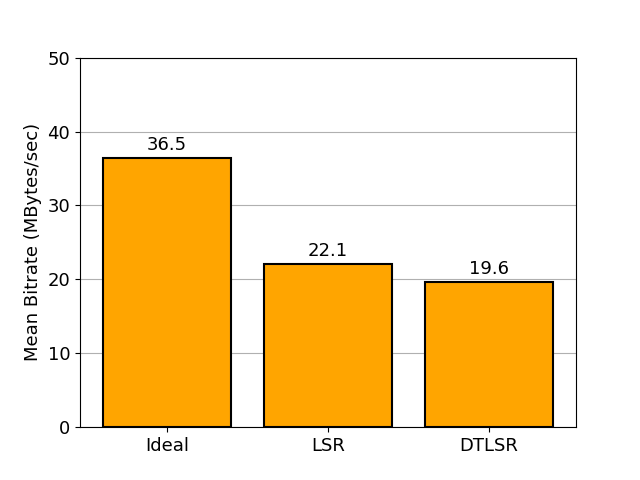
\includegraphics[width=0.8\linewidth]{tcp_bar_flap5_30}
  \caption{Throughput of TCP over unreliable network}
  \label{fig:tcp_5_30}
\end{figure}

Figure~\ref{fig:tcp_5_30} also shows that DTLSR has a slightly lower bitrate than LSR. I predict that this is due to DTLSR's buffering system and TCP's feedback system working very poorly with each other. When the link comes back up, a DTLSR router forwards all of the buffered packets as quickly as possible, resulting in a flood of ACKs being returned to the sender. TCP isn't designed expecting this to occur and so it introduces instability into its feedback system, reducing the mean bitrate overall as it tries to recover.

In both of the analyses described above, I show how TCP has an inherent weakness in running on a delay-tolerant network, particularly in responding correctly to the link coming back up. Thus, in real applications it is not simply enough to replace the routing layer of a traditional network stack, but the session layer as well must be changed in order to adapt to the new behaviour that the routing layer exhibits.


\section{Summary}

This chapter shows that DTLSR is an effective protocol for improving the delay and packet delivery in an unreliable network environment.

In particular, DTLSR has a strong advantage over LSR in maximising packet delivery in sparsely connected, unreliable networks, especially when link failures cause network partitions. I show further that the data loss caused by node failures has negligible impact on delays, thanks to the nLSA request mechanism. Even when backup links exist, DTLSR is shown to reduce the drop rate of packets by around half compared to LSR. DTLSR's largest advantage is shown in networks with correlated link failures leading to no end-to-end connection, providing a delivery rate upwards of 70\% compared to LSR providing no communication whatsoever.

I also show that the session-layer protocol running above the routing layer is critically important for taking advantage of the delay-tolerant characteristics in a real scenario. The commonly-used TCP responds badly to the inherent instability of a network like this, and so an awareness of the network stack as a whole is crucial when deploying a delay-tolerant system into the real world.

\chapter{Conclusion}

In this dissertation, I describe DTLSR, a routing protocol designed to maximise packet delivery and minimise delay for use in unreliable but topologically stable networks, and compare it to a traditional routing algorithm (LSR).

The project has been a success, fully meeting the initial goals and surpassing my expectations for performance.

\section{Achievements}

As described in Chapter~\ref{chapter:evaluation}, DTLSR surpasses LSR in a wide variety of unreliable networks. Figure~\ref{fig:partition_2_18} shows a case where the unreliable link is only up 10\% of the time; DTLSR achieves a drastically higher delivery rate than LSR, at 97\%. Even when a backup link exists---a case where I expected delay-tolerant modifications to have a minimal impact---DTLSR reduced the packet drop rate by more than half.

A fascinating case is detailed in Figure~\ref{fig:full_partition_flap20} where multiple link failures cause no end-to-end connection to exist. LSR achieved zero packet delivery, a critical problem that cannot be ameliorated with packet retransmission. DTLSR achieved more than 70\% delivery, which is an overwhelming success.

\begin{minipage}{0.5\textwidth}
\begin{figure}[H]
  %\hspace*{2.4cm}
  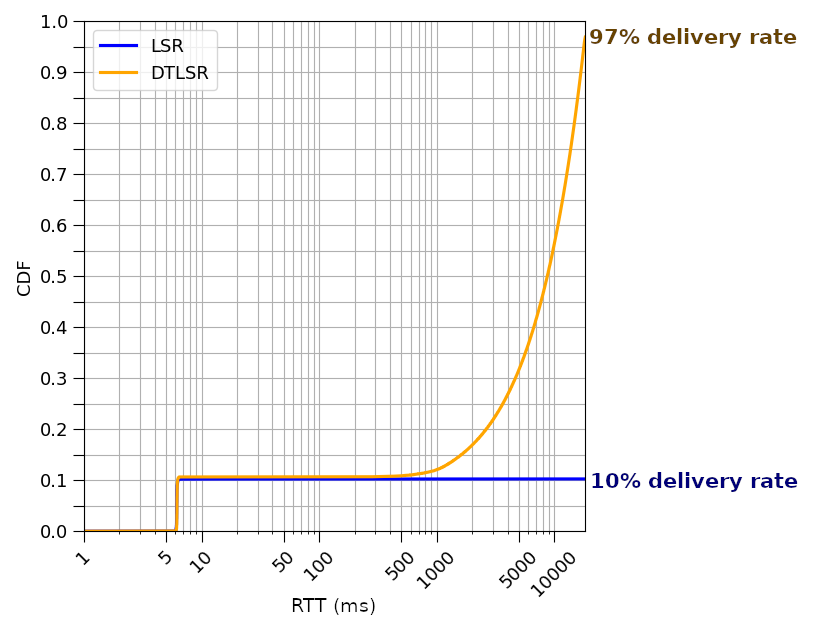
\includegraphics[width=1\linewidth]{delay_partition_flap2_18}
  \repeatcaption{fig:partition_2_18}{}
\end{figure}
\end{minipage}%
\begin{minipage}{0.5\textwidth}
\begin{figure}[H]
  %\centering
  %\hspace*{2.4cm}
  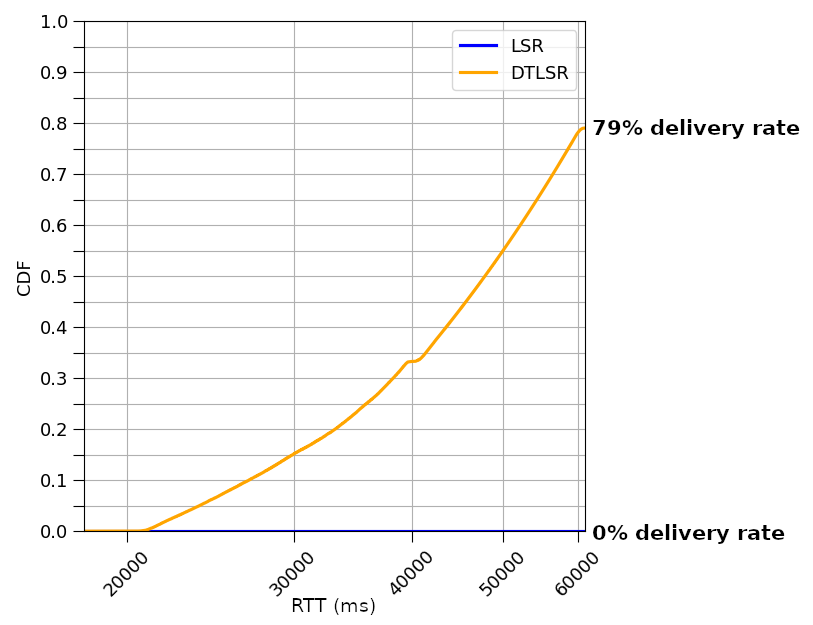
\includegraphics[width=1\linewidth]{delay_full_partition_flap20}
  \repeatcaption{fig:full_partition_flap20}{}
\end{figure}
\end{minipage}


\section{Lessons Learnt}

This project greatly tested my software engineering, systems engineering, and computer science abilities. I have found it a wonderful learning experience.

Choosing to implement the protocols in C taught me a lot about software development for a low-level, high-performance system. While C provided a few useful utilities used in this project, it would have been much easier to implement in a higher-level language, such as OCaml or Java; for example, I had particular pains with memory management, which these languages manage automatically. Due to the research nature of this project, of comparing two protocols rather than creating a production-ready implementation, if I were to start again, I would choose to implement it in one of these languages.

\section{Future Work}

Although DTLSR has met its goals, it could be enhanced further. While it is a much more proactive protocol than LSR, making general predictions about link reliability in the future with a single metric value, one could use more complex pattern recognition to predict exactly when the link will come back up based on its flapping behaviour in the past. This could be implemented with a simple statistical analysis of the uptime history but could also be extended to use machine learning techniques to detect more complex flapping patterns.

One could also test the two protocols in an unreliable network environment with real hardware, perhaps even in the field. Given the significant performance advantage shown by DTLSR over LSR in emulated network testing using CORE, it is promising enough that the costs would be worth it. CORE allows real nodes to be connected to the emulated network, reducing the marginal cost of testing in this way as it could be done incrementally, requiring minimal modification of the protocols.

As described in section~\ref{sec:tcp}, TCP has some severe deficiencies running atop a delay-tolerant routing layer. It would be very interesting to explore session-layer protocols that are more delay-tolerant, either adaptations of TCP or completely new designs. This is an exciting space for new ideas to be explored.



\bibliography{bibliography}

\appendix
\addtocontents{toc}{\protect\setcounter{tocdepth}{0}}

\chapter{Project Proposal}

\vspace{-8mm}
\Huge\textbf{Delay-Tolerant Link State Routing}

\vspace{8mm}
\LARGE\textbf{Introduction and Description of the Work}\normalsize

The network layer in the network stack handles the selection of a path across a network for packets to take, from node to node over connecting links. Small, static networks can use manually configured routing tables, but for large and/or dynamic networks this quickly becomes infeasible. Dynamic routing constructs routing tables automatically using information provided by a routing protocol.

The link state routing (LSR) protocol is one class of these, where every node attempts to construct a map of the entire network showing connectivity and other link properties. This map is used to construct the best path to every other node, which then forms the node’s routing table.

On a link going down, standard LSR will remove it from the map immediately (not considering propagation), potentially partitioning the network. However there are situations where we could expect these links to come back up relatively soon, in which case it would be better to forward the packets up until the break, and then have that node forward the packets once the link comes back up. This potentially makes more efficient use of network resources, depending on the judgement of whether links are truly down for good or not.

My project will be to implement a proposed modification of LSR, called delay-tolerant LSR, and investigate its viability. I will implement the OSPF LSR protocol, modify it to create a DTLSR protocol, and then compare the two.

\vspace{8mm}
\Large\textbf{Application}\normalsize

One area in which DTLSR is useful is in developing regions, whose network infrastructure can be very unreliable, leading to network partitions lasting minutes, hours, or days. DTLSR helps to make efficient use of limited resources and can often allow connectivity where no end-to-end connection ever exists.

\begin{figure}[H]
  \centering
  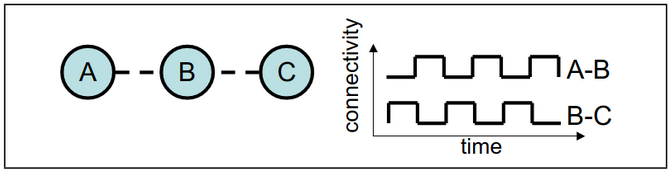
\includegraphics[width=0.8\linewidth]{proposal_1}
\end{figure}

\vspace{8mm}
\LARGE\textbf{Starting Point}\normalsize

I have no previous experience implementing or designing a network protocol, however I have studied the Computer Networking course in Part 1B, which covered the fundamentals of of routing protocols.

I will be using the Common Open Research Emulator (CORE), a network emulator. CORE requires that network services are written in C. As above I have never written a network service but I have done the C \& C++ course in Part 1B, as well as doing a summer internship writing C for embedded devices.

I have installed CORE on my machine to verify that it works. CORE includes a number of routing protocol suites such as Quagga, which includes full RFC implementations of OSPFv2 and OSPFv3. I will ignore these implementations and write my own limited version, so these are not included in the starting point.

\vspace{8mm}
\LARGE\textbf{Substance and Structure of the Project}\normalsize

First I will implement a version of the OSPF protocol into CORE as a network service running as a Unix routing daemon. This version will contain only the functionality needed to generate routing tables, for example a graph representation, Link-State Announcement (LSA) messaging, graph merging to use most recent information, and graph searching to find the ‘shortest’ path to every other node.

\begin{figure}[H]
  \centering
  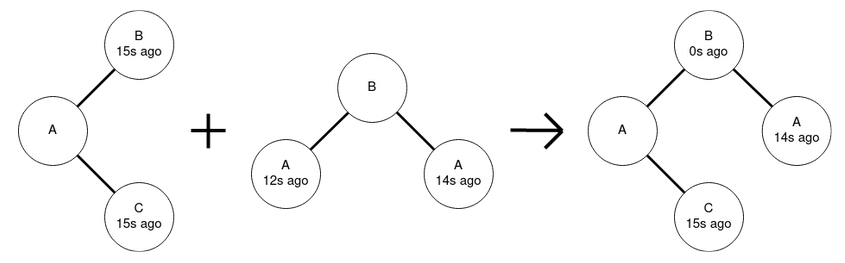
\includegraphics[width=0.9\linewidth]{proposal_2}
\end{figure}

Here node A has received an LSA from B, and merged the two graphs to use the most recent information.

I will then extend the implementation with the delay-tolerant modifications described above. One particular modification is of the path cost of links. In OSPF it is a function of bandwidth, but I will modify this to instead minimise the expected delay. in up links this will use information like the bandwidth and the size of the packet queue, but in down links we can estimate the delay by using a sliding window over the uptime history to estimate the delay (i.e.\ when the link will come back up).

\begin{figure}[H]
  \centering
  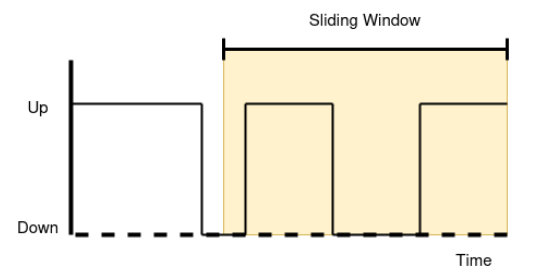
\includegraphics[width=0.6\linewidth]{proposal_3}
\end{figure}

Another modification is that of when forwarding decisions are made. Typically the forwarding decision is made on packet arrival, where it is then placed in a queue for that outgoing interface. However in our scenarios packets can be in the queue for hours, by which time the network may have changed and that forwarding decision is no longer the best. We can instead use `per-contact’ routing, where all packets are in a single queue and forwarding decisions can be made every time a new contact is detected, potentially `short-circuiting’ the routing decision to take advantage of the good timing of a link coming back up, and sending packets that suddenly have a new, much quicker route than originally predicted.

\vspace{8mm}
\LARGE\textbf{Possible Extensions}\normalsize

\begin{itemize}
\item
Add support for dynamic scaling of protocol parameters to adapt to changing network conditions, for example increasing the size of the sliding window when a consistent connection `schedule’ is detected with minimal unexpected fluctuation.

\item
Investigate how queue capacity at nodes impacts the number of dropped packets, as buffer overflow will be the main cause of packet loss.

\item
Utilise machine learning techniques for predicting when links will come back up.
\end{itemize}

\vspace{8mm}
\LARGE\textbf{Success Criteria}\normalsize

For the project to be deemed a success the following items must be successfully completed.

\begin{enumerate}
\item
Design and implement the core routing functionality of OSPF as a CORE network service.

\item
Design and implement a delay-tolerant LSR as a modification of the above OSPF implementation as a CORE network service.

\item
Create a series of simulation scenarios to evaluate my implementations and compare their performance.
\end{enumerate}

To measure the success of items 1 and 2, as stated in the evaluation section below I will ensure that packets are correctly routed through a multi-hop network in CORE. I will consider the project a success if both the OSPF and DTLSR protocols are fully functional, as the point of the project is to evaluate the effectiveness of delay-tolerant modifications.

\vspace{8mm}
\LARGE\textbf{Evaluation}\normalsize

To evaluate my protocol implementations, I will use the CORE network emulator. This allows me to generate many different network layouts as well as scripting network traffic and changing network conditions over time. This will typically mean varying the connection status of links.

My model of connection patterns will attempt only to model independent link failures, and not a targeted attack on the network. I will however model scenarios where these independent failures lead to a network partition, for example.

CORE allows network statistics to be gathered. I will compute the following metrics:

\begin{itemize}
\item
The percentage of dropped messages

\item
The percentage of a packet’s total lifetime spent enqueued at nodes

\item
Data throughput
\end{itemize}

Network utilisation as a measure of efficiency
These will be gathered for both OSPF and DTLSR in order to compare the performance of both and see whether DTLSR is statistically significantly more performant in low-reliability scenarios, as well as whether the changes made impact performance in more reliable networks.

I will ignore link bandwidths, as the frequency of links going up or down is practically always low enough such that a newly up link is always up long enough to empty the queue at the node.

\vspace{8mm}
\LARGE\textbf{Timetable and Milestones}\normalsize

At some point I have to write the progress report, but the dates are not on the CST website. I also don’t know which particular date I should `start’ on for the timetable. 18th? 25th?

\large\textbf{Weeks 1-2} (25th October - 7th November)\normalsize\\
I will research the operation and implementation of network services, as well as how they are implemented in CORE as Unix routing daemons.

\large\textbf{Weeks 3-4} (8th November - 21st November)\normalsize\\
I will begin the implementation of OSPF as a CORE network service by designing and implementing the graph representation of the network, as well as the algorithm for merging graphs together using LSA messages to get the most recent map of the network.

\large\textbf{Weeks 5-6} (22nd November - 5th December)\normalsize\\
I will finish implementing graph merging and implement the graph searching algorithm to compute the `shortest’ paths to every other node. This will be verified by a suite of unit tests. I will start planning the comparative evaluation of the two protocols, generating different scenarios and working out how test data can be read from CORE.

\large\textbf{Weeks 7-8} (6th December - 19th December)\normalsize\\
I will finish the OSPF implementation and verify that it works using CORE’s functionality for sending packets between nodes. I will also begin designing the DTLSR protocol, and modifying the OSPF protocol to implement it.

\large\textbf{Weeks 9-10} (20th December - 2nd January)\normalsize\\
Two weeks of relaxation over Christmas, and catching up on behind work if need be.

\large\textbf{Weeks 11-12} (3rd January - 16th January)\normalsize\\
I will finish the implementation of the DTLSR protocol, verifying that it works like I did for OSPF, and then include it in the evaluation process. This crucially allows comparison between the two protocols, which could inspire new evaluation techniques and metrics that I didn’t originally think of.

\large\textbf{Weeks 13-15} (17st January - 6th February)\normalsize\\
I will write the progress report, catch up on any implementation work I am behind on and if time allows continue with evaluation.

\large\textbf{Weeks 16-17} (7th February - 20th February)\normalsize\\
I will start the formal writeup of the dissertation, completing the introduction and preparation chapters. Evaluation will continue.

\large\textbf{Weeks 18-19} (21st February - 6th March)\normalsize\\
I will complete the implementation chapter, continuing with evaluation.

\large\textbf{Weeks 20-21} (7th March - 20th March)\normalsize\\
I will complete the evaluation and conclusion chapters by the end of these two weeks.

\large\textbf{Weeks 22-23} (21st March - 3rd April)\normalsize\\
Buffer time for extra work I need to do if I fall behind, as well as time for my supervisor to read over the dissertation and make corrections as needed.

\large\textbf{Weeks 24-25} (4th April - 17th April)\normalsize\\
Make corrections and final changes to the dissertation.

\vspace{8mm}
\LARGE\textbf{Resources Required}\normalsize

I will use my personal laptop of develop this project; a Lenovo Ideapad L340, with a 2.6 GHz Intel Core i7-9750H CPU and 16 GB of RAM. I accept full responsibility for this machine, and its function for the duration of my project. Should my laptop become unusable, I will switch to using the provided MCS computers. I will prevent data loss by hosting my project and dissertation on GitHub, whilst also making regular offline backups with a 64GB USB stick.

I plan on using CORE, available on the Linux platform, to test the protocols and to aid in their implementation. It is available on GitHub under a bespoke licence suitable for a Part II project.

I will write the network services in C, and so will require a GCC C compiler, widely available on all platforms under the GPL licence.

\vspace{8mm}
\LARGE\textbf{Papers and Useful Links}\normalsize

Practical Routing in Delay-Tolerant Networks (https://dl.acm.org/doi/pdf/10.1145/1080139.1080141)

Delay Tolerant Routing for Developing Regions (http://kfall.com/papers/dtlsr-nsdr07.pdf)

Services in CORE (https://www.brianlinkletter.com/2014/11/core-network-emulator-services-overview/\#more-2914)

CORE service customisation (https://www.brianlinkletter.com/2014/11/how-to-customize-core-network-emulator-services/)

Writing a network service (https://sites.google.com/site/tfsidc/create-a-network-service)

OSPFv2 RFC (https://datatracker.ietf.org/doc/html/rfc2328)

Quagga Routing Suite (https://www.quagga.net/)




\addtocontents{toc}{\protect\setcounter{tocdepth}{2}}
%%%%%%%%%%%%%%%%%%%%%%%%%%%%%%%%%%%%%%%%%%%%%%%%%%%%%%%%%%%%%%%%%%%%%%%%%%%%%%%%
%% Index:
%%
%\printthesisindex

\end{document}

